%!TEX root = ../thesis.tex
%*******************************************************************************
%****************************** Second Chapter *********************************
%*******************************************************************************

\chapter{Methods}

\ifpdf
    \graphicspath{{Chapter2/Figs/Raster/}{Chapter2/Figs/PDF/}{Chapter2/Figs/}}
\else
    \graphicspath{{Chapter2/Figs/Vector/}{Chapter2/Figs/}}
\fi
In this chapter we introduce all the methods we used in this project. The explanations are not exhaustive but act as a good primer if more details are of interested.
In the first section we present ordination methods, which are very frequently used as part of exploratory data analysis in ecological studies. We use them to sketch plots and search for patterns in our data and also as dimensionality reduction techniques.

The classical hypothesis test permutational multivariate analysis of variance is introduced in the following section. It is used to check if the groupings of samples along the levels of a categorical variable significantly different from each other. A distance metric is used to quantify the dissimilarity between samples, and a permutation scheme to avoid assuming the F-statistic's distribution. 

Classification models are introduced in the next section together with a brief outline of their working. In particular, the models presented are Logistic Regression and Random Forest. A Bayesian interpretation of the former is also given which can be implemented with Markov chain Monte Carlo methods.  

An outline of the Hamiltonian Monte Carlo method for sampling from normalisable distributions is given in the final section of this Chapter. We motivate its use by transforming the problem of sampling to physics terms. Then, we introduce Hamiltonian dynamics and their properties which allow for an efficient exploration of the state space of the target distribution.

\section{Ordination}
\label{sec:ordination}
Ordination can be thought of as series of operations/transformations performed on a data matrix (samples and species table) with the purpose of representing the relationships between the species and samples as faithfully as possible. These methods are made up of two stages; the data are converted into a dissimilarity/similarity matrix of the samples or species and are subsequently transformed into a lower dimensional space where the interpoint distances are related to the distance matrix through the scaling method used.

Metric scaling methods try to maximise the linear correlation between the distances in the dissimilarity matrix and in the lower dimensional space. Non-metric methods on the other hand aim at maximising rank-order correlation between those distances instead.

Some of the reasons for carrying out ordination are :
\begin{itemize}
\item To make the dissimilarities between the sites or species more evident in a visual manner.
\item To reduce the noise from the data, since the projection of the ordination method used will be of a lower dimensional space.
\item To interpret environmental gradients along the dimensions.
\end{itemize}


Ordination methods can be categorised based on how they use external environmental variables; when the method only considers the sites by species table then it is classified as indirect gradient analysis (or unconstrained ordination), when it takes in to account environmental data from the start then it is classified as direct gradient analysis (or constraint ordination). 

Indirect gradient analysis finds the most important gradients in the sites by species data (or more descriptive dimensions), in the absence of environmental data. After the procedure is complete, environmental gradients can be fitted on the new basis and explore how the variables change with sites or species. Direct gradient analysis on the other hand explores how much environmental variables are related to the variation of species composition across sites, by taking into consideration only the variation that can be explained by the environmental variables. It can be thought of as a regression technique testing the null hypothesis that the species composition is not related to environmental gradients.

%%PCA
\subsection{Principal Components Analysis}
\label{ssec:PCA}
Principal Component analysis (PCA) is a clustering technique that can be used as an ordination method as well. It works by finding the direction that explains the most variance in the data and setting it as the first axis. Then it finds the direction with the second highest explanation of variance that is orthogonal to the first one, and sets it as the second axis, and the direction that is uncorrelated with both the first and the second axis and explains the most variance as the third, and so on. For ordination, since all ecological community data are measured in the same units, the data do not need to be standardised to unit variance, and thus the method involves finding the eigenvectors of the covariance matrix of the data (and not the correlation matrix).

Let the row vector $x_i$ with $p$ columns represent the $i$th sample of our data, with each element denoting how many individuals of that particular column (species/OTU) are encountered in the sample. We can place the vectors into an $n \times p$ matrix $X$, where $n$ is the number of samples collected. For ecological abundance data we only have to centre the data by finding the mean abundance of each species and subtracting it from matrix $X$:
\begin{align}
\label{eq:columnmean}
u_j &= \frac{1}{n} \sum_{i = 1}^{n} X_{ij} \\
B &= X - h u^T,
\end{align}
where  $u_j$ is the $p\times 1$ vector of mean values, $h$ is a $n \times 1$ vector of ones and $B$ is the centred matrix. This expression can be rewritten  using the $n \times n$ centering matrix $J$ which is defined as
\begin{align}
J = I - \frac{1}{n}O,
\end{align}
where $I$ is the identity matrix and $O$ is $n \times n$ matrix of ones. Multiplying this matrix on the left with $X$ produces the same result as centering the matrix by columns
\begin{equation}
B = JX.
\end{equation}
The $p\times p$ empirical covariance matrix is then computed as
\begin{equation}
C = \frac{B^T B}{n},
\end{equation}
which is diagonalised to find its eigenvectors and eigenvalues \cite{franklin_matrix_2012}
\begin{equation}
C = VDV^{-1},
\end{equation}
where $D$ is the diagonal matrix with the eigenvalues of $C$ in its diagonal, and $V$ is the matrix with the eigenvectors of $C$ as its columns. The projections of the data onto the eigenvectors is given by 
\begin{equation}
Y = BV.
\end{equation}
To reduce the number of features, we can select the $m$ eigenvectors of $C$ that correspond to the $m$ largest eigenvalues, sort them in decreasing order (so the first column of $V$ corresponds to the eigenvector with the largest eigenvalue, the second column to the second largest eigenvalue and so on), and create a new matrix of the sorted eigenvectors
\begin{align}
W_{ij} = V_{ij} \text{ where i = 1,...,$p$ and j = 1,...,$m$}.
\end{align}
Then the projection to the reduced eigenvector space is given by
\begin{equation}
Y_r = BW,
\end{equation}
which is a $n \times m$ matrix.
%Gramm MAtrix
When the number of features $p$ is greater than the number of observations $n$, it is computationally more efficient to diagonalise the Gram matrix $G$ to find the eigenvectors of $C$
\begin{equation}
\label{eq:gram}
G = \frac{BB^T}{n}.
\end{equation}
The Gram matrix has dimensions $n \times n$ and can be diagonalised to give 
\begin{equation}
G = USU^{-1}.
\end{equation}
In this instance, $U$ columns are the eigenvectors of the Gram matrix. The connection between this diagonalisation and of the Covariance matrix can be seen more clearly through the singular value decomposition of $B$
\begin{equation}
B = U \Sigma V^T,
\end{equation}where $U$ and $V$ are $n \times n$ and $p \times p$ matrices respectively with orthogonal unit vectors as columns. The matrix $\Sigma$ is an $n \times p$ rectangular diagonal matrix of positive numbers, the singular values of $B$. Using this representation of $B$, we can rewrite the covariance and Gram matrix as such
\begin{align}
C &= \frac{B^TB}{n} = \frac{(U\Sigma V^T)^TU\Sigma V^T}{n} = \frac{V\Sigma^T U^TU\Sigma V^T}{n} = \frac{V \Sigma^T\Sigma V^T }{n} \\
G &= \frac{BB^T}{n} = \frac{U\Sigma V^T(U\Sigma V^T)^T}{n} = \frac{U\Sigma V^TV\Sigma^T U^T}{n} = \frac{U\Sigma \Sigma^T U^T}{n}.
\end{align}
Since matrices $U$ and $V$ are orthogonal,  their inverse is equal to their transpose (e.g. $U^{-1} = U^T$) \cite{franklin_matrix_2012}. The projection of the centred data onto the eigenvectors of the covariance matrix $C$ can be reformulated using the SVD
\begin{align}
Y = BV = U \Sigma V^T V = U \Sigma.
\end{align}
This reformulation tells us that the projections can also be found using the eigenvectors of the Gram matrix (i.e. the left-singular vectors of $B$). The projection to the reduced $m$-dimensional eigenvector space can be given in a similar manner by
\begin{align}
\label{eq:reducedGram}
Y_r = U_m \Sigma_m,
\end{align}
where $\Sigma_m$ is the matrix of the $m$ largest singular values, and $U_m$ the matrix with their corresponding eigenvectors as columns.

The centred $n \times p$ data matrix $B$ has maximum rank $r$ equal to the minimum of the numbers $n$ and $p$. This means that there are at most $r$ linearly independent row (or column) vectors, and consequently, at most $r$ singular values in the $n \times p$ matrix $\Sigma$. Comparing the two decompositions of the Covariance and Gram matrix, we note that the matrices $\Sigma^T \Sigma$ and $\Sigma \Sigma^T$ have the same number of non-zero elements in their diagonals, even if they are of dimension $p \times p$ and $n \times n$ respectively. Thus, we can conclude that the Covariance and Gram matrices have the same eigenvalues.



%Principal component analysis (PCA) is a statistical procedure that uses an orthogonal transformation to convert a set of observations of possibly correlated variables (entities each of which takes on various numerical values) into a set of values of linearly uncorrelated variables called principal components. This transformation is defined in such a way that the first principal component has the largest possible variance (that is, accounts for as much of the variability in the data as possible), and each succeeding component in turn has the highest variance possible under the constraint that it is orthogonal to the preceding components. The resulting vectors (each being a linear combination of the variables and containing n observations) are an uncorrelated orthogonal basis set. PCA is sensitive to the relative scaling of the original variables.

An important assumption of PCA is that there are linear relationships between all the features. Therefore, the principal components are constructed such that they decouple the linear correlations between them. This assumption, however, makes it unsuitable for use in Ecological data sets. The species composition varies non linearly across samples, and the relationship between species is also not linear. The presence of a species in a sample is usually much more important that the actual number of read counts of that species. Thus, when the data are projected onto the eigenvectors of the covariance matrix (Figure \ref{fig:pcaotu12}), they are distorted into a horseshoe shape (i.e. like an arch) \cite{gauch_noise_1982}. PCA was performed using the rda function in the Vegan package \cite{oksanen_vegan_nodate,oksanen_multivariate_nodate}.

%FIGURE OF PCA
\begin{figure}
\centering
\includegraphics[width = 0.7\textwidth]{"pcaotu12"}
\caption{First 2 dimensions of PCA performed on the full OTU table. The 2 axes account for 47.8\% of the variance.}
\label{fig:pcaotu12}
\end{figure}

%%PCOA
\subsection{Principal Coordinates Analysis}
A more general method of ordination, of which PCA is a special case, is called Principal Coordinates Analysis (PCoA), otherwise known as classical multidimensional scaling. The method aims to represent dissimilarities between samples (in the species space) in a lower dimensional space, so that they can be easily interpreted. This is done by creating a distance matrix using whatever metric we wish (with the condition that it returns a scalar given two vectors of arbitrary dimensions) that quantifies the dissimilarities between our samples. The data are then projected to a lower dimensional space by maximising the linear correlation between the distances in the distance matrix and the inter-point distances in the lower dimensional projection. Thus, the method assumes that the distances used are meaningful and thus try to reserve them. It was first introduced by Torgerson in 1952 as a tool in psychometrics \cite{torgerson_multidimensional_1952}.

Lets define by $D_{ij}$ the $n \times n$ distance matrix between the samples (rows) in $X$ (where $D_{ij}$ indicates the distance between sample $i$ with $j$). It is evident from its construction that it is symmetric, since the distance between sample $i$ and $j$ is the same as the distance between $j$ and $i$. When using a euclidean metric to quantify the distance the diagonals are zero. The euclidean metric is given by
\begin{align}
D_{ij} = {||\mathbf{x}_i- \mathbf{x}_j||},
\label{eq:euclideanmetric}
\end{align}
where $ \mathbf{x}_i$ is a row vector of the data matrix $X$ containing the abundance reading for the sample $i$, and $||\cdot||$ is the L2 norm.

The algorithm first double centres the element squared distance matrix $D^2$, or in other words subtracts the row and column mean, and multiplying it by $-\frac{1}{2}$
\begin{align}
\label{eq:Kmatrix}
K = -\frac{1}{2}JD^2J.
\end{align}
Then the matrix $K$ is decomposed into its eigenvectors, which are the columns of matrix $E$, and eigenvalues, which make up the diagonals of matrix $\Lambda$
\begin{equation}
    K = E\Lambda E
\end{equation}

The $m$ largest eigenvalues with their corresponding eigenvectors are collected and sorted in a descending manner in matrices $E_m$ and $\Lambda_m$ (so the largest eigenvalue is $\Lambda_{m,11}$ with corresponding eigenvector $E_{m,{ \bullet}1}$, the first column of the $E_m$ matrix). The projection of the data onto the reduced $m$-dimensional space is given by
\begin{align}
Y_r = E_m \Lambda_m^{(1/2)},
\end{align}
where the exponent is applied element-wise on all eigenvalues (the square root of each eigenvalue is used). This representation looks very similar to the one obtained in equation \ref{eq:reducedGram}, where the projection is calculated using the eigenvectors of the Gram matrix. We will show how, when using an Euclidean metric, PCoA is equivalent to PCA.

We can expand the euclidean distance matrix into 
\begin{align}
D^2_{ij} &= ||\mathbf{x}_i - \mathbf{x}_j||^2 = ||\mathbf{x}_i - \mathbf{\bar{x}}+\mathbf{\bar{x}} -\mathbf{x}_j||^2   \\
&= ||\mathbf{x}_i - \mathbf{\bar{x}}||^2 + ||\mathbf{x}_j - \mathbf{\bar{x}}||^2 - 2(\mathbf{x}_i - \mathbf{\bar{x}})\cdot (\mathbf{x}_j - \mathbf{\bar{x}}),
\end{align}
where the last term is the dot product between the vectors of the mean-centred samples $i$ and $j$. The $||\mathbf{x}_i - \mathbf{\bar{x}}||^2$ term is an additive constant over the columns of $D_{ij}$, and so is the corresponding term with $\mathbf{x}_j$ over the rows of the matrix.  To uncover the connection between the last term and the Gram matrix, we have to reformulate the later to an equivalent representation of the former. 


The mean centred matrix $B$ can be interpreted as row vectors $\mathbf{x}_i - \mathbf{\bar{x}}$ stacked on top of each other vertically. As before, $\mathbf{x}_i$ denotes the row vector of data matrix $X$ (i.e. the species abundance of sample $i$) and $\mathbf{\bar{x}}$ denotes the row vector with the mean number of reads of each species across all samples
\begin{equation}
\mathbf{\bar{x}} = [u_1,u_2,...,u_p], 
\end{equation}
where $u_j$ is defined as in equation \eqref{eq:columnmean}. To construct the Gram matrix, we multiply the mean-centred matrix with its transpose
\begin{equation}\frac{1}{n}
\brows{(x_1 - \bar{x})\\(x_2 - \bar{x})\\ \rowsvdots \\(x_n - \bar{x})} \cdot 
\begin{pmatrix}
\vert &\vert&&\vert\\
\text{\begin{sideways}$(x_1 - \bar{x})$
\end{sideways}}&
\text{\begin{sideways}$(x_2 - \bar{x})$
\end{sideways}}& 
\hdots&
\text{\begin{sideways}$(x_n - \bar{x})$
\end{sideways}}\\
\vert&\vert &&\vert 
\end{pmatrix}= \frac{1}{n}
\begin{pmatrix}
(x_1-\bar{x})\cdot (x_1-\bar{x}) &\hdots&(x_1-\bar{x}) \cdot (x_n-\bar{x}) \\
(x_2-\bar{x}) \cdot (x_1-\bar{x})&\hdots&(x_2-\bar{x}) \cdot (x_n-\bar{x})\\
\vdots&\ddots&\vdots\\
(x_1-\bar{x})\cdot (x_n-\bar{x})&\hdots&(x_n-\bar{x})\cdot (x_n-\bar{x})
\end{pmatrix},
\end{equation}
and get the expression 
\begin{equation}
G_{ij} =\frac{1}{n}(x_i-\bar{x}) \cdot (x_j-\bar{x}). 
\end{equation}
The Gram matrix rows' and columns' means are equal to zero since it is double-centred by construction
\begin{align}
G = \frac{1}{n}BB^T = \frac{1}{n}JX(JX)^T =\frac{1}{n} JXX^TJ^T = \frac{1}{n}JG_{uc}J,
\end{align}
where $J$ is the centring matrix (which  is symmetric), and $G_{uc}$ the uncentered Gram matrix. Therefore, when we double centre the Distance matrix, we end up with the Gram matrix scaled by a constant number
\begin{align}
JD_{ij}J&= J\left(||x_i - \bar{x}||^2 + ||x_j - \bar{x}||^2 - 2nG_{ij}\right)J \\
&\propto -2G_{ij}\\
K &\propto G,
\end{align}
Where $K$ is the matrix we decompose into its eigenvalues and eigenvectors in the PCoA method (equation \eqref{eq:Kmatrix}). The two terms preceding the Gram matrix go to zero when double-centred since they are constants over rows and columns. As mentioned earlier, the Gram matrix itself stays the same when double centred since its rows' and columns' mean is zero. 

Therefore, diagonalising the $K$ matrix when using a euclidean distance metric (PCoA method) is equivalent to diagonalising the Gram matrix of the mean-centred data. The projections produced by the two methods are the same since the eigenvector ($E$ for PCoA and $U$ for PCA) and eigenvalue ($\Lambda^{(1/2)}$ for PCoA and $\Sigma $ for PCA) matrices are the same. 

%IF TIME DO THIS
%Another, more intuitive, way to view PCoA is geometrically. It amounts to creating a multidimensional object using the distance matrix, and then applying orthogonal transformations to it to obtain 
%Other distance metrics
%~~~~~~~~~~~~~~~~~~~~~~~~~~~~~~~~~~~~~~
A Euclidean distance metric, however, is not very useful when it comes to ecological abundance data. This is because it suffers from the same drawbacks that PCA does (see earlier discussion in section \ref{ssec:PCA}). The framework of PCoA was developed so as to enable the use of other measures which are more suitable to ecological data; as mentioned earlier, the number of read counts for each species might suffer from biases and thus not much emphasis should be place on their value. Such a measure is the Bray-Curtis dissimilarity statistic, which quantifies how dissimilar two samples are by taking the absolute value of their difference. The measure $B_{ij}$ is defined as
%~~~~~~~~~~~~~~~~Bray Curtis
\begin{equation}
    B_{ij} = \frac{\sum_{k =1}^{p} |X_{ik} - X_{jk}|}{\sum_{k =1}^{p} X_{ik} + X_{jk}},
\end{equation}
where $X_{ik}$ is the data matrix which denotes the number of reads of speciment $k$ in sample $i$. The statistic ranges from 0, where the samples have the same species composition, to 1 where the samples do not have any species in common, and is semimetric\footnote{Semimetric measures do not satisfy the triangle inequality.}. If the data matrix is instead made up of presence and absence values (1 if an OTU was found in a sample, 0 otherwise), the Bray-Curtis index quantifies the fraction of species not in common between the samples. 

If we use this statistic to calculate the distance matrix $D_{ij}$ and then carry out PCoA, the arch effect is absent from the 2 dimensional ordination plot and can better separate the different river samples. As it can be seen in Figure \ref{fig:pcoaotu12}, the method can separate well samples from the upper Maranon part of the river (yellow points in the upper right corner of the plot). Samples from other parts are grouped together on the opposite side from the upper Maranon points. Black and white river samples are not very well separated, and occupy the same space (except on the upper right corner where no black water samples are found). Even when the ordination method produces a better spread of results than when using PCA, the variance explained by the first 2 axes is only 19.8\%.


%% PCoA bray curtis.
\begin{figure}[h]
\centering
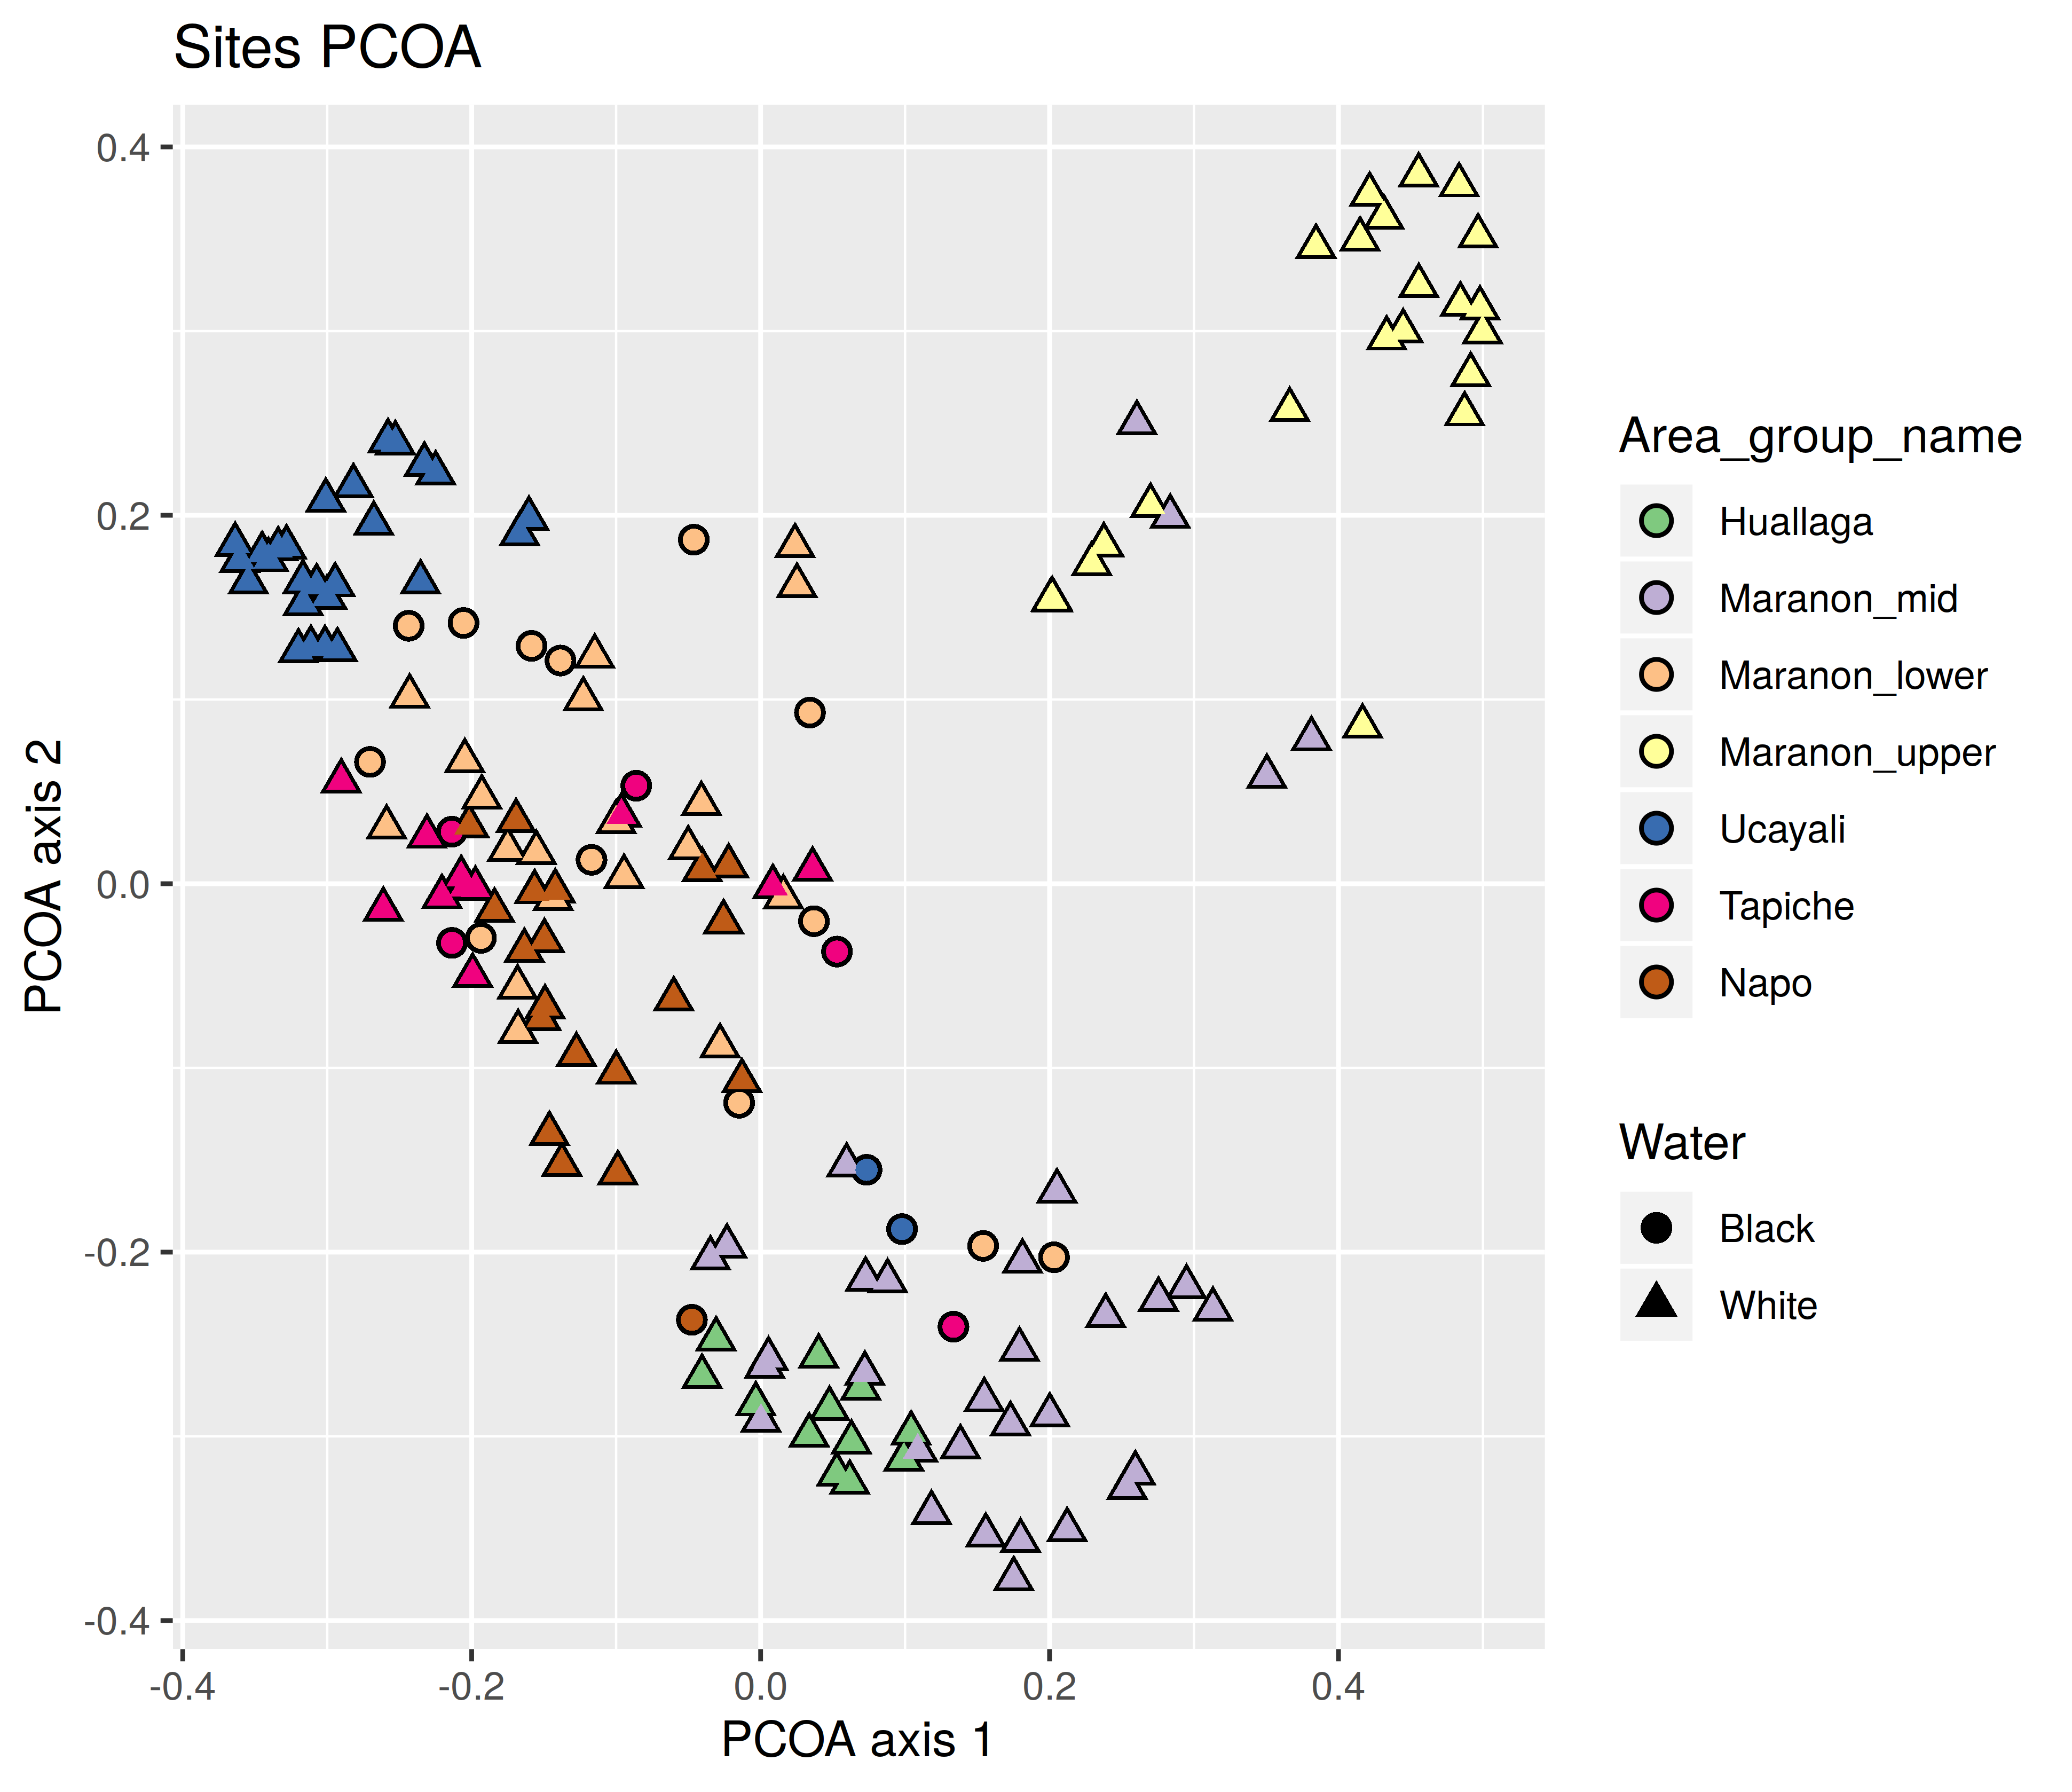
\includegraphics[width = 0.7\textwidth]{pcoaotu12}
\caption{First 2 dimensions of PCoA performed on the full OTU table using the Bray Curtis statistic as the distance metric. The 2 axes account for 19.8\% of the variance.}
\label{fig:pcoaotu12}
\end{figure}

To illustrate the effect of measures on the PCoA algorithm, we produced 2 dimensional ordination plots for the Euclidean and the Jaccard metrics. The Euclidean metric has the form given in equation \eqref{eq:euclideanmetric} and the ordination plot (see Figure \ref{fig:pcoaeuc}) has the same form as the one obtained using PCA. The only difference is the scale (the covariance matrix is divided by the number of samples) and the reflection of the points on the x-axis. The Jaccard metric is given by
\begin{equation}
Jac_{ij} =\frac{2C_{ij}}{1-C_{ij}},
\end{equation} 
where $C_{ij}$ is the Bray-Curtis statistic between sample $i$ and $j$. The ordination plot produced using this index is shown in Figure \ref{fig:pcoajac}. PCoA was performed using the pcoa function in the ape package in R \cite{paradis_ape_nodate}.

%%RESULTS of PCoA with different metrics
\begin{figure}[h]
\centering
\begin{subfigure}{0.4\textwidth}
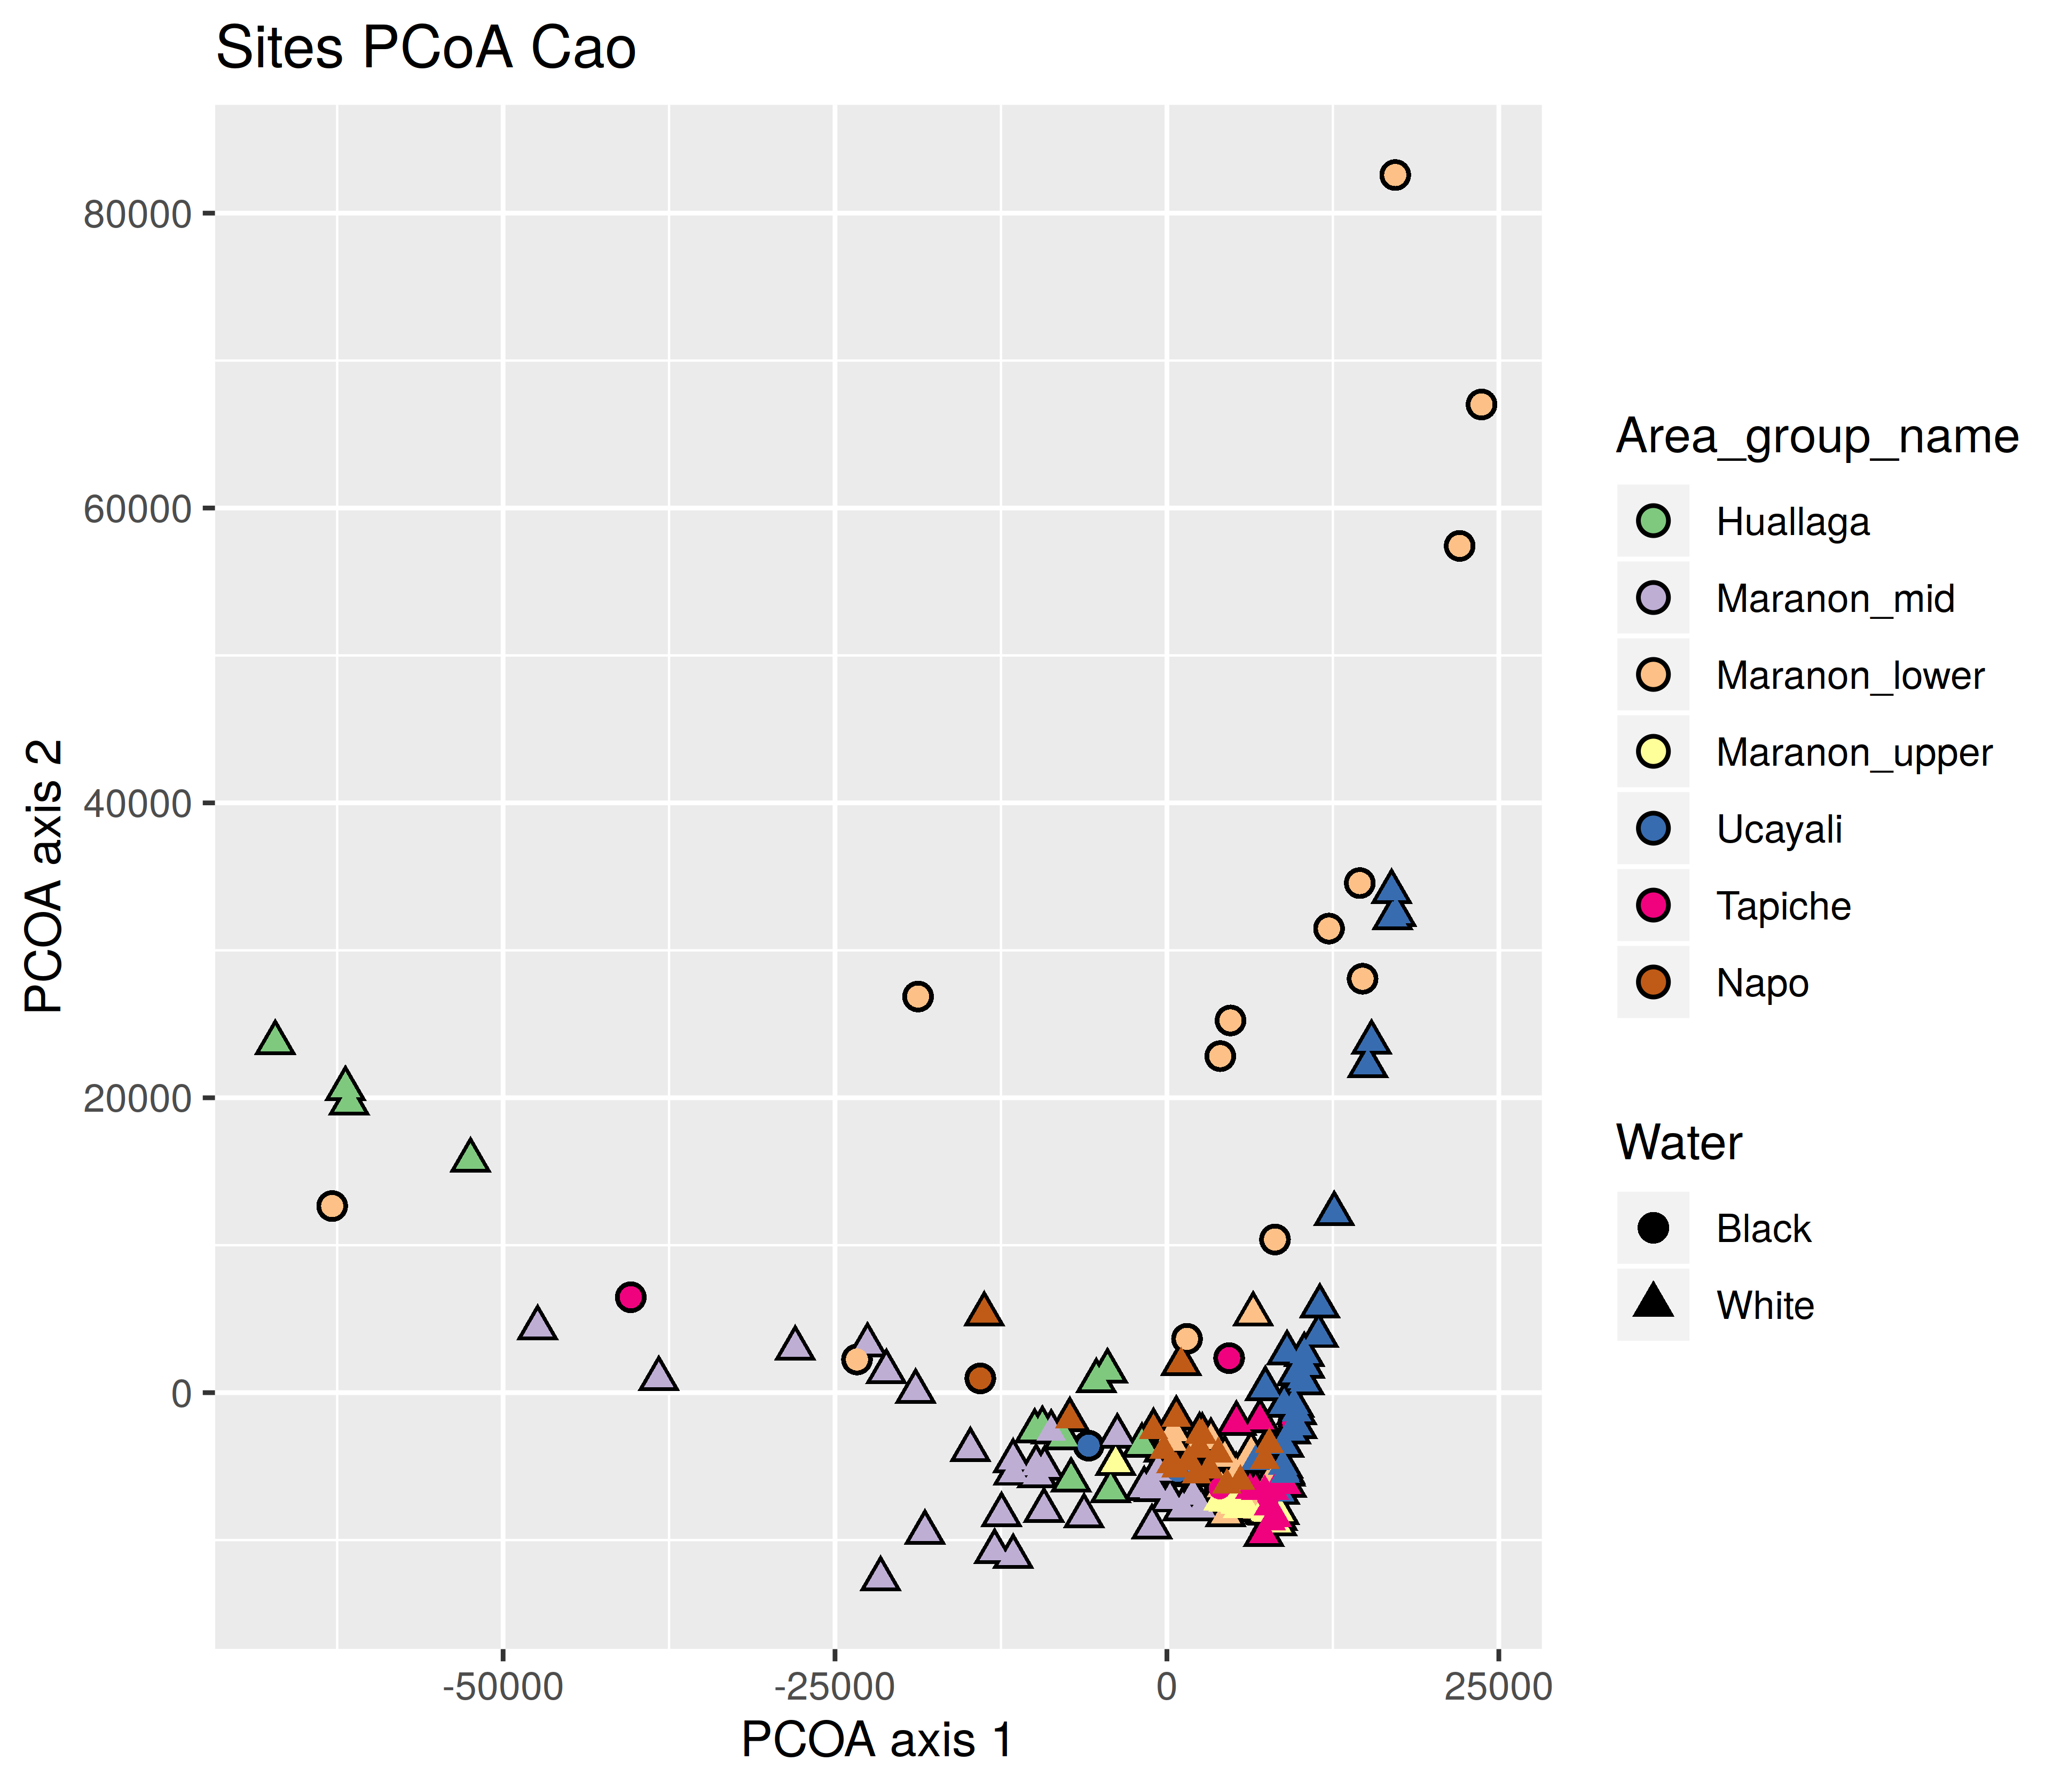
\includegraphics[width = \textwidth]{pcoa12eucotu}
\caption{}
\label{fig:pcoaeuc}
\end{subfigure}
\begin{subfigure}{ 0.4\textwidth}
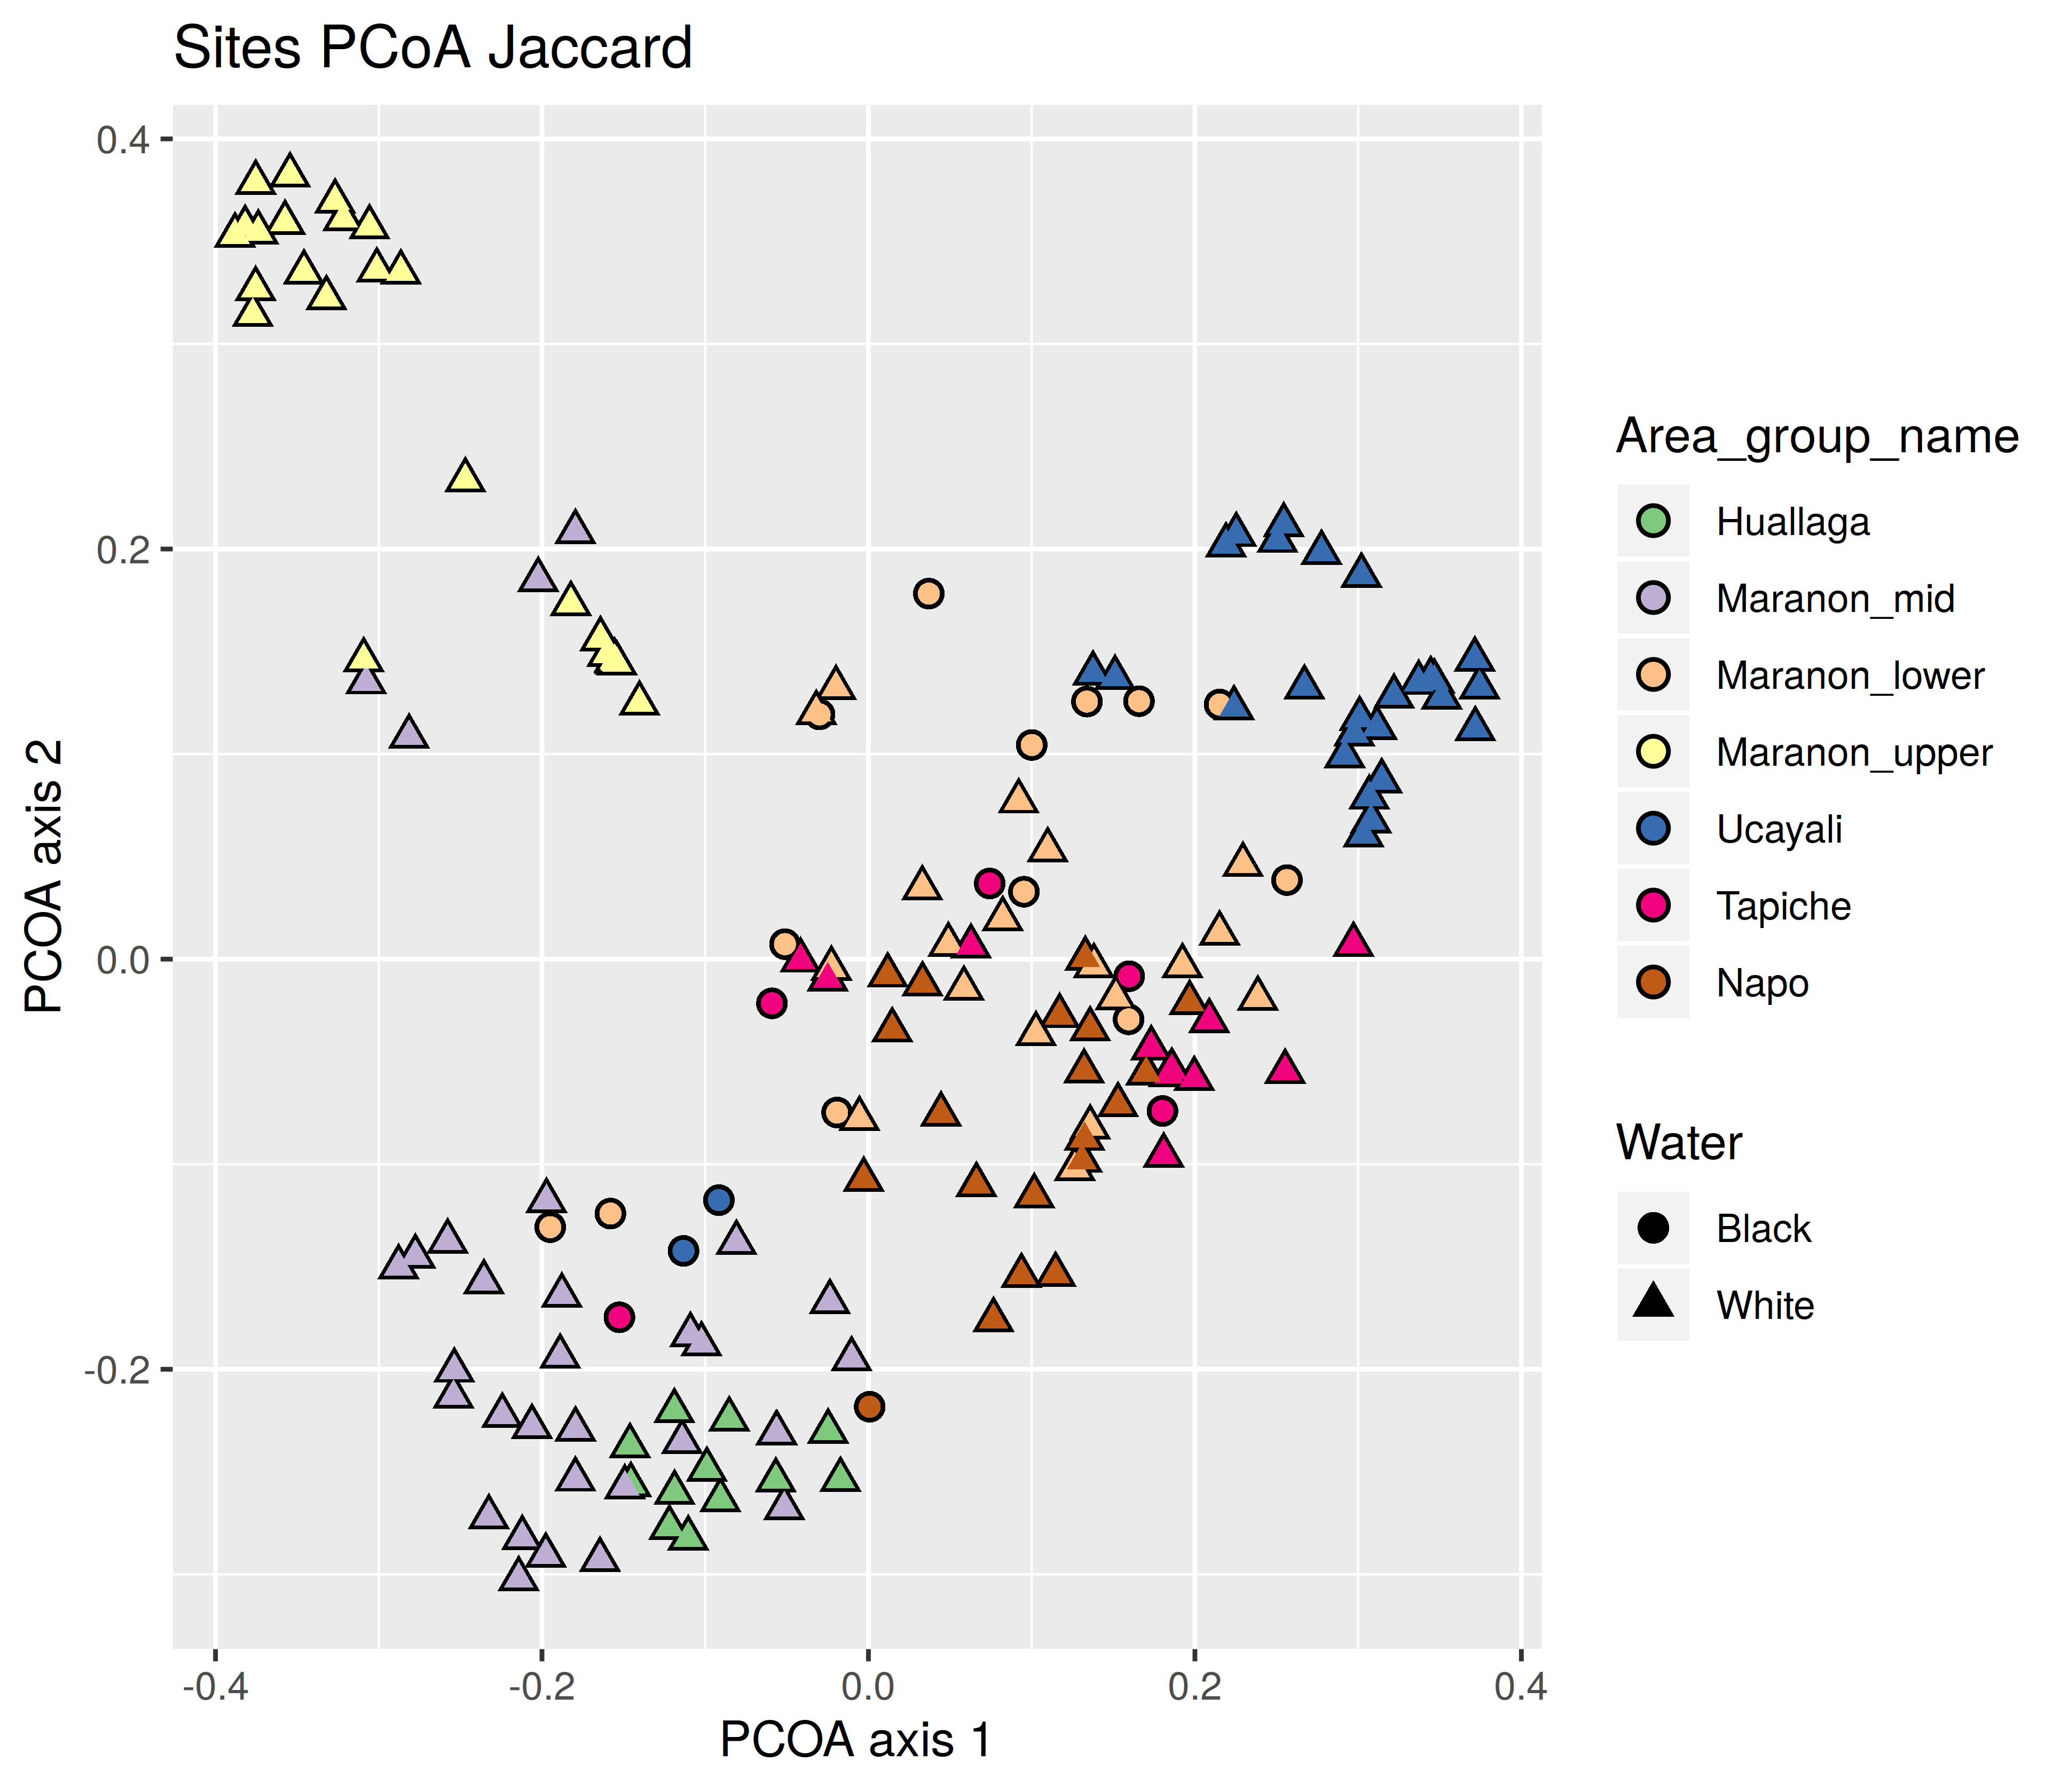
\includegraphics[width = \textwidth]{pcoa12jacotu}
\caption{}
\label{fig:pcoajac}
\end{subfigure}
\caption{PCoA using the Euclidean \ref{fig:pcoaeuc}  and Jaccard \ref{fig:pcoajac} metric. The result for the Euclidean metric is the same as with PCA; only the scales have different values and the points are flipped over the X-axis. The Jaccard metric produces a similar result with Bray-Curtis since they are rank-order similar.}
\end{figure}
%Motivate NMDS
%EG actual distances are not that important so NMDS might be more usefull which maximisies correlation
%% NMDS
%%%Explain similarity of NMDS with PCOA

% Uncomment this line, when you have siunitx package loaded.
%The SI Units for dynamic viscosity is \si{\newton\second\per\metre\squared}.
% \begin{figure}[htbp!] 
% \centering    
% \includegraphics[width=1.0\textwidth]{minion}
% \caption[Minion]{This is just a long figure caption for the minion in Despicable Me from Pixar}
% \label{fig:minion}
% \end{figure}
\subsection{Non-metric multidimensional scaling}
Non-metric multidimensional scaling (NMDS) is distinct from classical multidimensional scaling methods, like PCA and PCoA, in that it does not assume there is a linear relationship between the actual ecological distance of two samples and their dissimilarity (e.g. using Bray-Curtis). In contrast it assumes only that there is a rank order relationship between the two (i.e. the most different samples should also have the largest dissimilarity). Thus, it derives a configuration of points representing the samples, in which the inter-point distance of the pairs are in rank order with the dissimilarities of the samples.
Furthermore, it is a random iterative approach and the number of dimensions of the configuration of points must be decided from beforehand. Like PCoA, NMDS was first introduced in the psychometrics field for use in psychology \cite{kruskal_multidimensional_1964}.
%%PCoA and so-called 'classical' multidimensional
%scaling (Torgerson, 1952) assume that the dissimilarity measure has a linear relationship with ecological distance. In contrast, nonmetric multidimensional scaling (NMDS, Shepard, 1962a, b; Kruskal,
%1964a, b) assumes only rnonotonicity: a configuration is derived in which the distances between sample pairs are in rank order with their dissimilarities. 

The goal of the algorithm is to find $n$ points in an $m$ dimensional spaces whose inter-point distances are somewhat related to the experimental dissimilarities of our $n$ objects/samples. In this instance, dissimilarity is given by the distance matrix between samples $\Delta_{ij}$ which is calculated using a dissimilarity measure. In NMDS ordination we are not interested in the numerical distance between our objects but rather their ordinal relationship (the rank of dissimilarities between samples is of importance); that's why the word dissimilarity is used. In contrast, PCoA or classical MDS assume a linear relationship between the calculated dissimilarity measure and the ecological distances of the samples. What we label as distance ${D}_{ij}$ in NMDS is between the points in the $m$ dimensional projection of our object. A measure of relatedness between distance and dissimilarity is given by a goodness-of-fit statistic which is an integral part of the procedure; in classical MDS however no such statistic is used.

This statistic is called Stress and it measures how the configuration of points in the $m$ dimensional space match the data, through a monotonic relationship between them. A solution to the iterative algorithm, the best-fitting configuration of points, is found when the stress is minimised. The best solution is achieved when there is a perfect monotone relationship between the dissimilarities and distances. 

The dissimilarities we are dealing with are symmetric; $\Delta_{ij} =\Delta_{ji}$. Therefore, only the upper triangular matrix is needed without the diagonal (because samples are perfectly similar between themselves). We want to achieve a configuration of points in an $m$ dimensional space such that the rank ordering of dissimilarities
\begin{equation}
	\Delta_{i_1 j_1} \leq 	\Delta_{i_2 j_2} \leq ... \leq 	\Delta_{i_M j_M},
	\label{eq:mon}
\end{equation}
where $M = \frac{n(n-1)}{2}$ is the number of interactions between the samples, is matched by the rank ordering of distances $D_{ij}$.

The objects are represented by points/vectors in an $m$-dimensional space ${ \mathbf x}_i \in \mathbb{R}^m$ or by the matrix $X_{ij}$, and their distance by any metric we want. In this case we choose the Euclidean:
\begin{equation}
	D_{i j}=\sqrt{\sum_{k=1}^{i}\left(X_{i k}-X_{j k}\right)^{2}}.
\end{equation}


An important element of the procedure are the numbers $\hat{D}_{ij}$, which are used as proxies for the dissimilarities when it comes to calculating the stress. The reason we do not use the numerical values of the dissimilarities is because we are not interested in them, only in their rank order relationship. Thus, the numbers $\hat{D}_{ij}$ are constructed as such to be monotonically related to $\Delta_{ij}$; when arranged in the order
\begin{equation}
	\hat{D}_{i_1 j_1},	\hat{D}_{i_2 j_2}, ...,	\hat{D}_{i_M j_M},
\end{equation}
each number is greater than or equal to the one before it. 
These numbers are chosen so as to be as `nearly equal' to $D_{ij}$ as possible, while satisfying the monotonicity of $\Delta_{ij}$ \eqref{eq:mon}. 


Now we can introduce the stress formula for a configuration of points $X_{ij}$. This is given by
\begin{align}
	S(X_{ij})&= \text{stress of the fixed configuration } { \mathbf x_1, ...,x_n}\\
	 &=\underset{\text{numbers }\hat{D}_{ij} \text{ satisfying \eqref{eq:mon}}}{ min}
	 \sqrt{\frac{\sum_{i<j}\left(D_{ij},-\hat{D}_{i j}\right)^{2}}{\sum_{i<j} D_{i j}^{2}}},
	 \label{eq:stress}
\end{align}
where the sum is taken over all $ij$ pairs such that $i<j$ is satisfied (sum over all upper triangular matrix elements), and the minimum is over the numbers $\hat{D}_{ij}$. This minimisation can also be seen as monotonic regression, if the dissimilarities $\Delta_{ij}$ are plotted against the distances $D_{ij}$ and the proxies are the points that make up the free-form line. The regression step is finding new $\hat{D}_{ij}$ numbers when the distances change. 

The algorithm then aims at finding the configuration of points that minimises \eqref{eq:stress}. The minimisation over the configuration is done by a `method of gradients' (similar to gradient descent) outlined in \cite{kruskal_nonmetric_1964}. That over the $\hat{D}_{ij}$ is done using a method of blocks outlined in \cite{miles_complete_1959,kruskal_nonmetric_1964}.


The algorithm first starts by generating a random configuration of $n$ non-identical points that span an $m$-dimensional space. This can also be done by running another ordination method and using it's configuration of points limited to the $m$ first dimensions. This set is then normalised; the centre of gravity is set to the origin, and the points are uniformly stretched or shrank such that their root-mean-square distance from the origin is equal to one. This transformation does not affect the algorithm since the euclidean metric is invariant to translations and rotations, and the denominator of stress also makes it invariant to a uniform stretch of the points. 

 The interpoint distance $D_{ij}$ is then calculated and the stress for the configuration is found by minimising the dissimilarity proxies  $\hat{D}_{ij}$ in the way described earlier. Then, the gradient of the configuration is calculated and, if some stopping conditions are not met that signify the algorithm reached an appropriate minimum, the points are moved towards the direction of decreasing stress. A new configuration is thus obtained and the procedure is repeated until some minimum conditions are met; either the stress is low enough that finding another minimum would not improve the solution significantly, or several attempts from different starting configurations have been attempted and the lowest stress solution is chosen. 

NMDS ordination was performed using the metaMDS function in vegan \cite{oksanen_vegan_nodate} package for R. As mentioned previously, the number of dimensions have to be predetermined before running the algorithm. There is also a maximum number of iteration to try if a non-convergent solution is found. Ordination plots for Bray-Curtis and Euclidean dissimilarity measures are shown in Figures \ref{fig:nmds} and \ref{fig:nmdseuc}. The same legends and colouring schemes have been used as in the PCoA case. The Bray-Curtis measure can separate river colour much better than when using the Euclidean measure. 


The stress of the 2 dimensional NMDS configuration was 15.8\% and 12.8\% for Bray-Curtis and Euclidean respectively. This is considered `fair' in the literature, and is good enough for discerning patterns in a plot. With increasing dimensions the stress falls, however, the number of iterations needed to get a convergent solution also increases considerably. After 100000 iterations a convergent solution for 20 dimensions was not found. Thus, its inclusion as a feature selection method might not be warranted. 

\begin{figure}[h]
	\centering
	\begin{subfigure}{0.45\textwidth}
		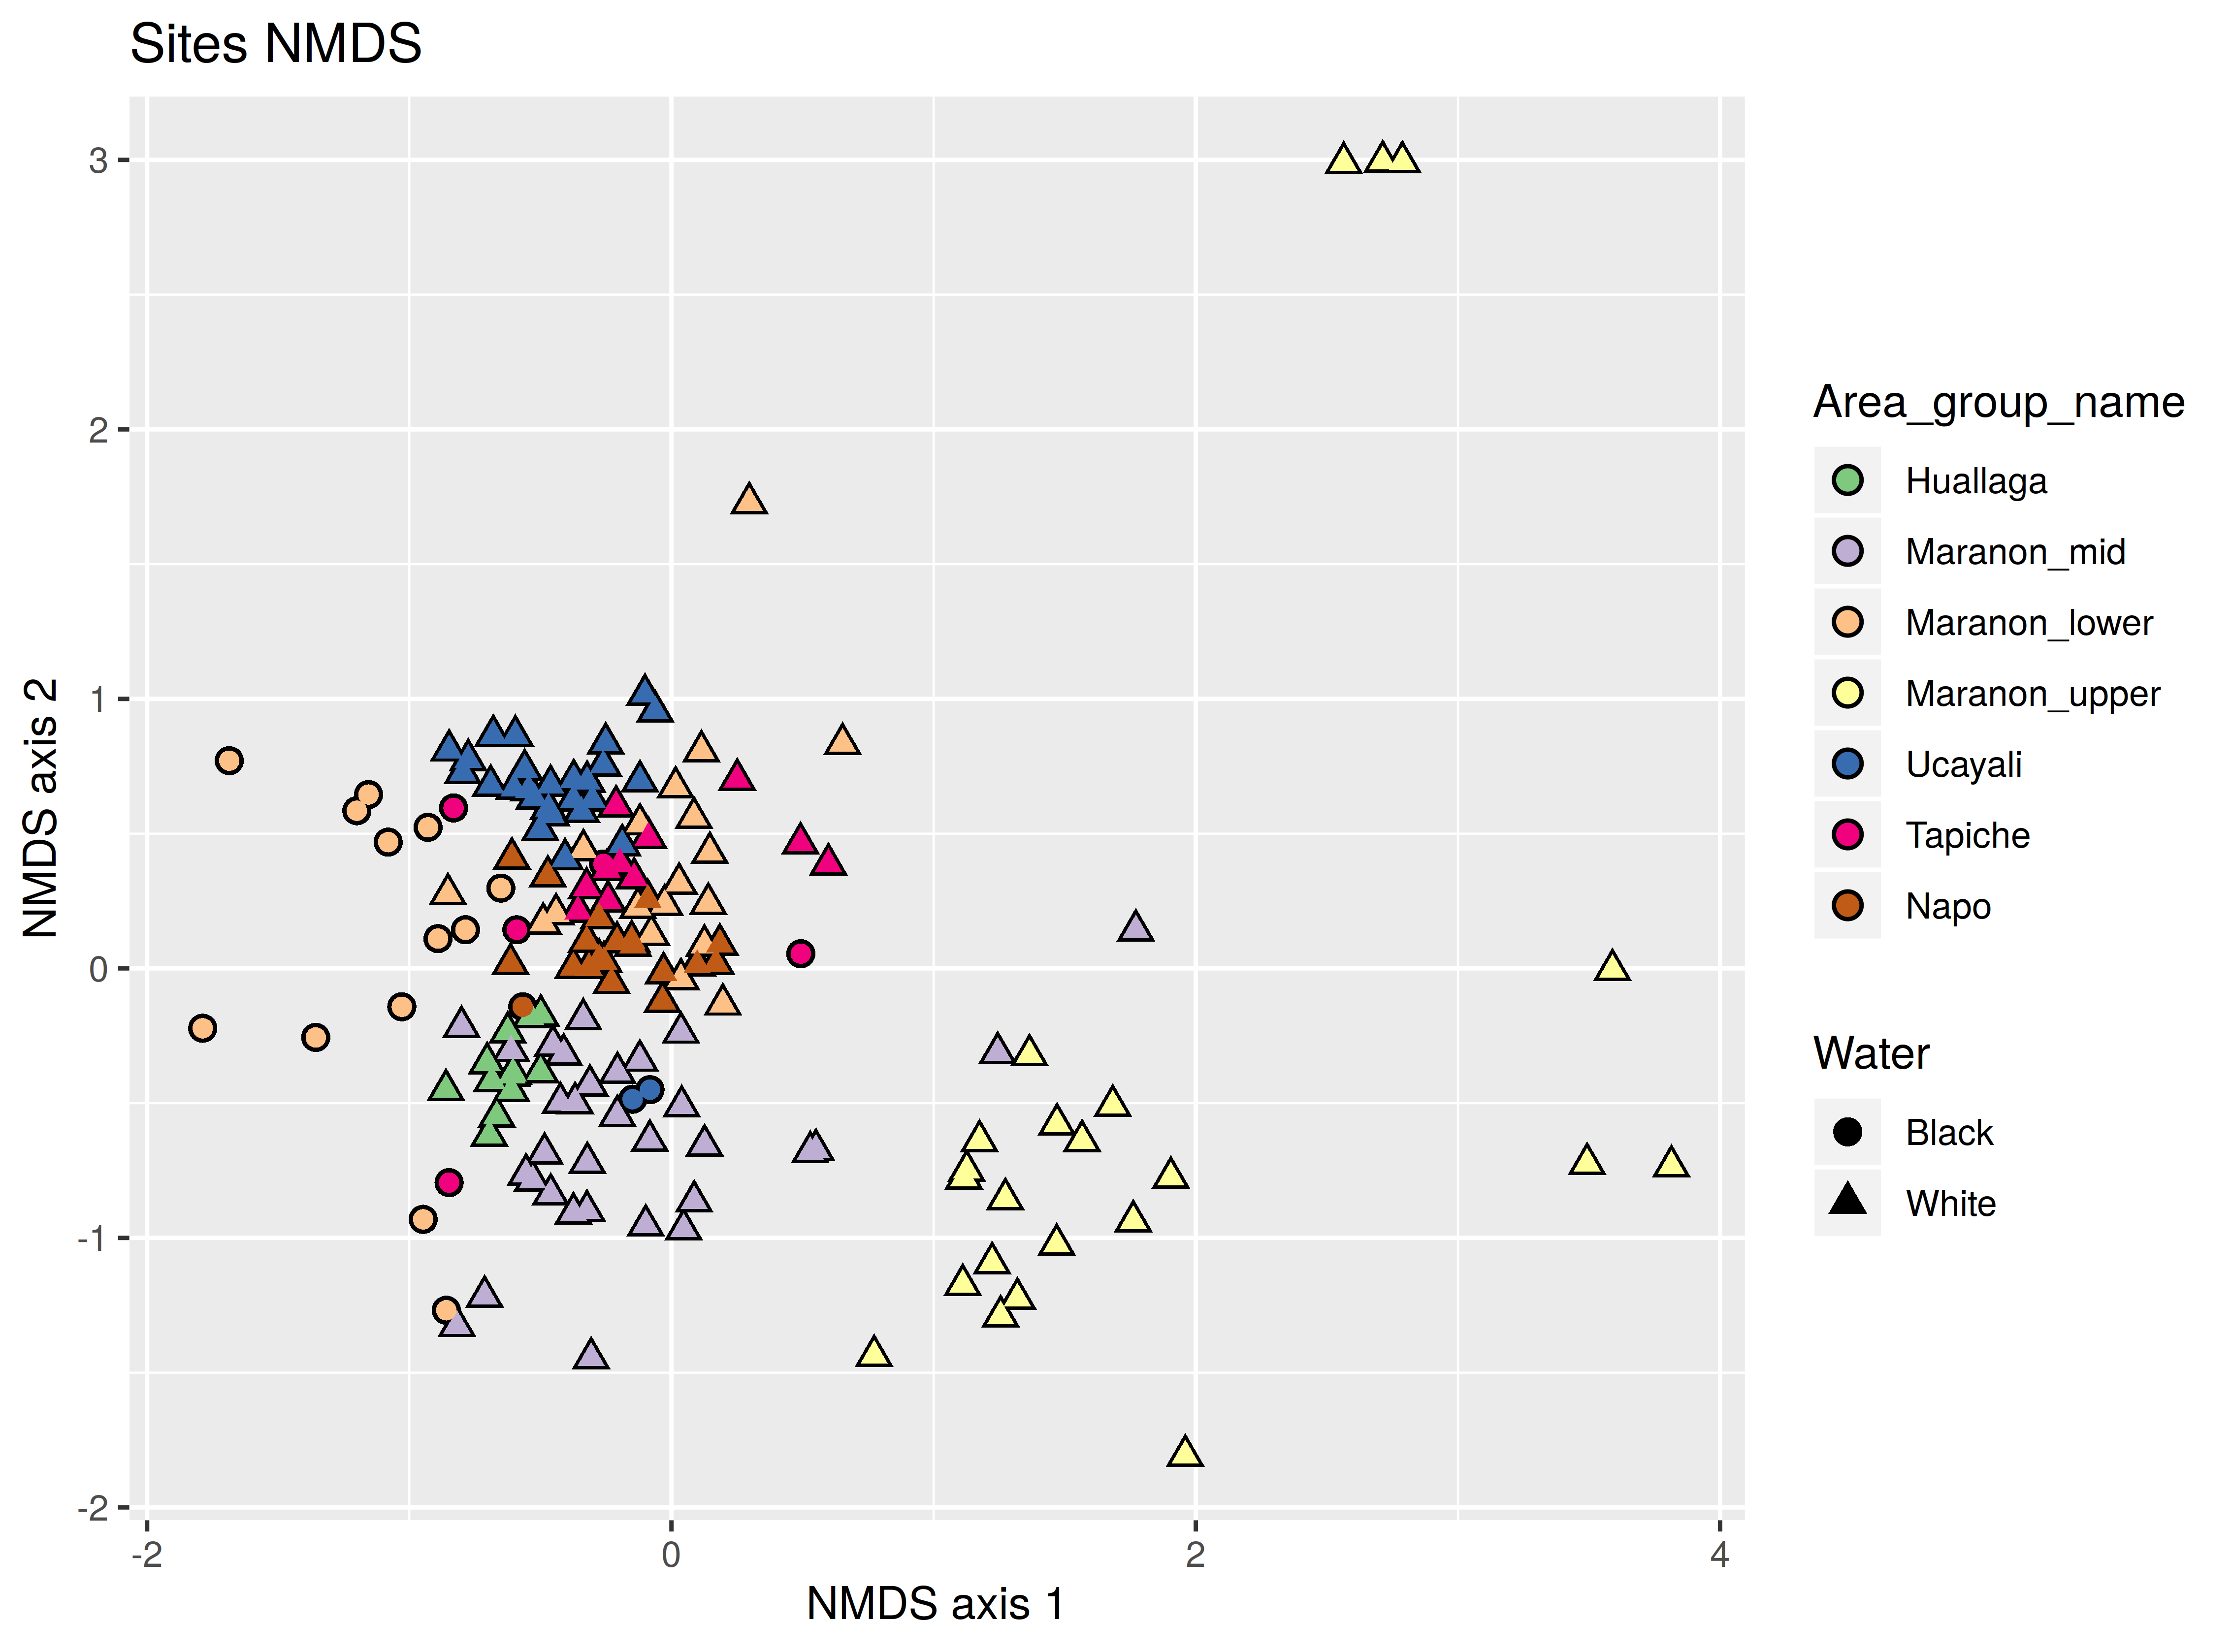
\includegraphics[width=\textwidth]{nmdsotu12}
		\caption{}
		\label{fig:nmds}
	\end{subfigure}
	\begin{subfigure}{0.45\textwidth}
		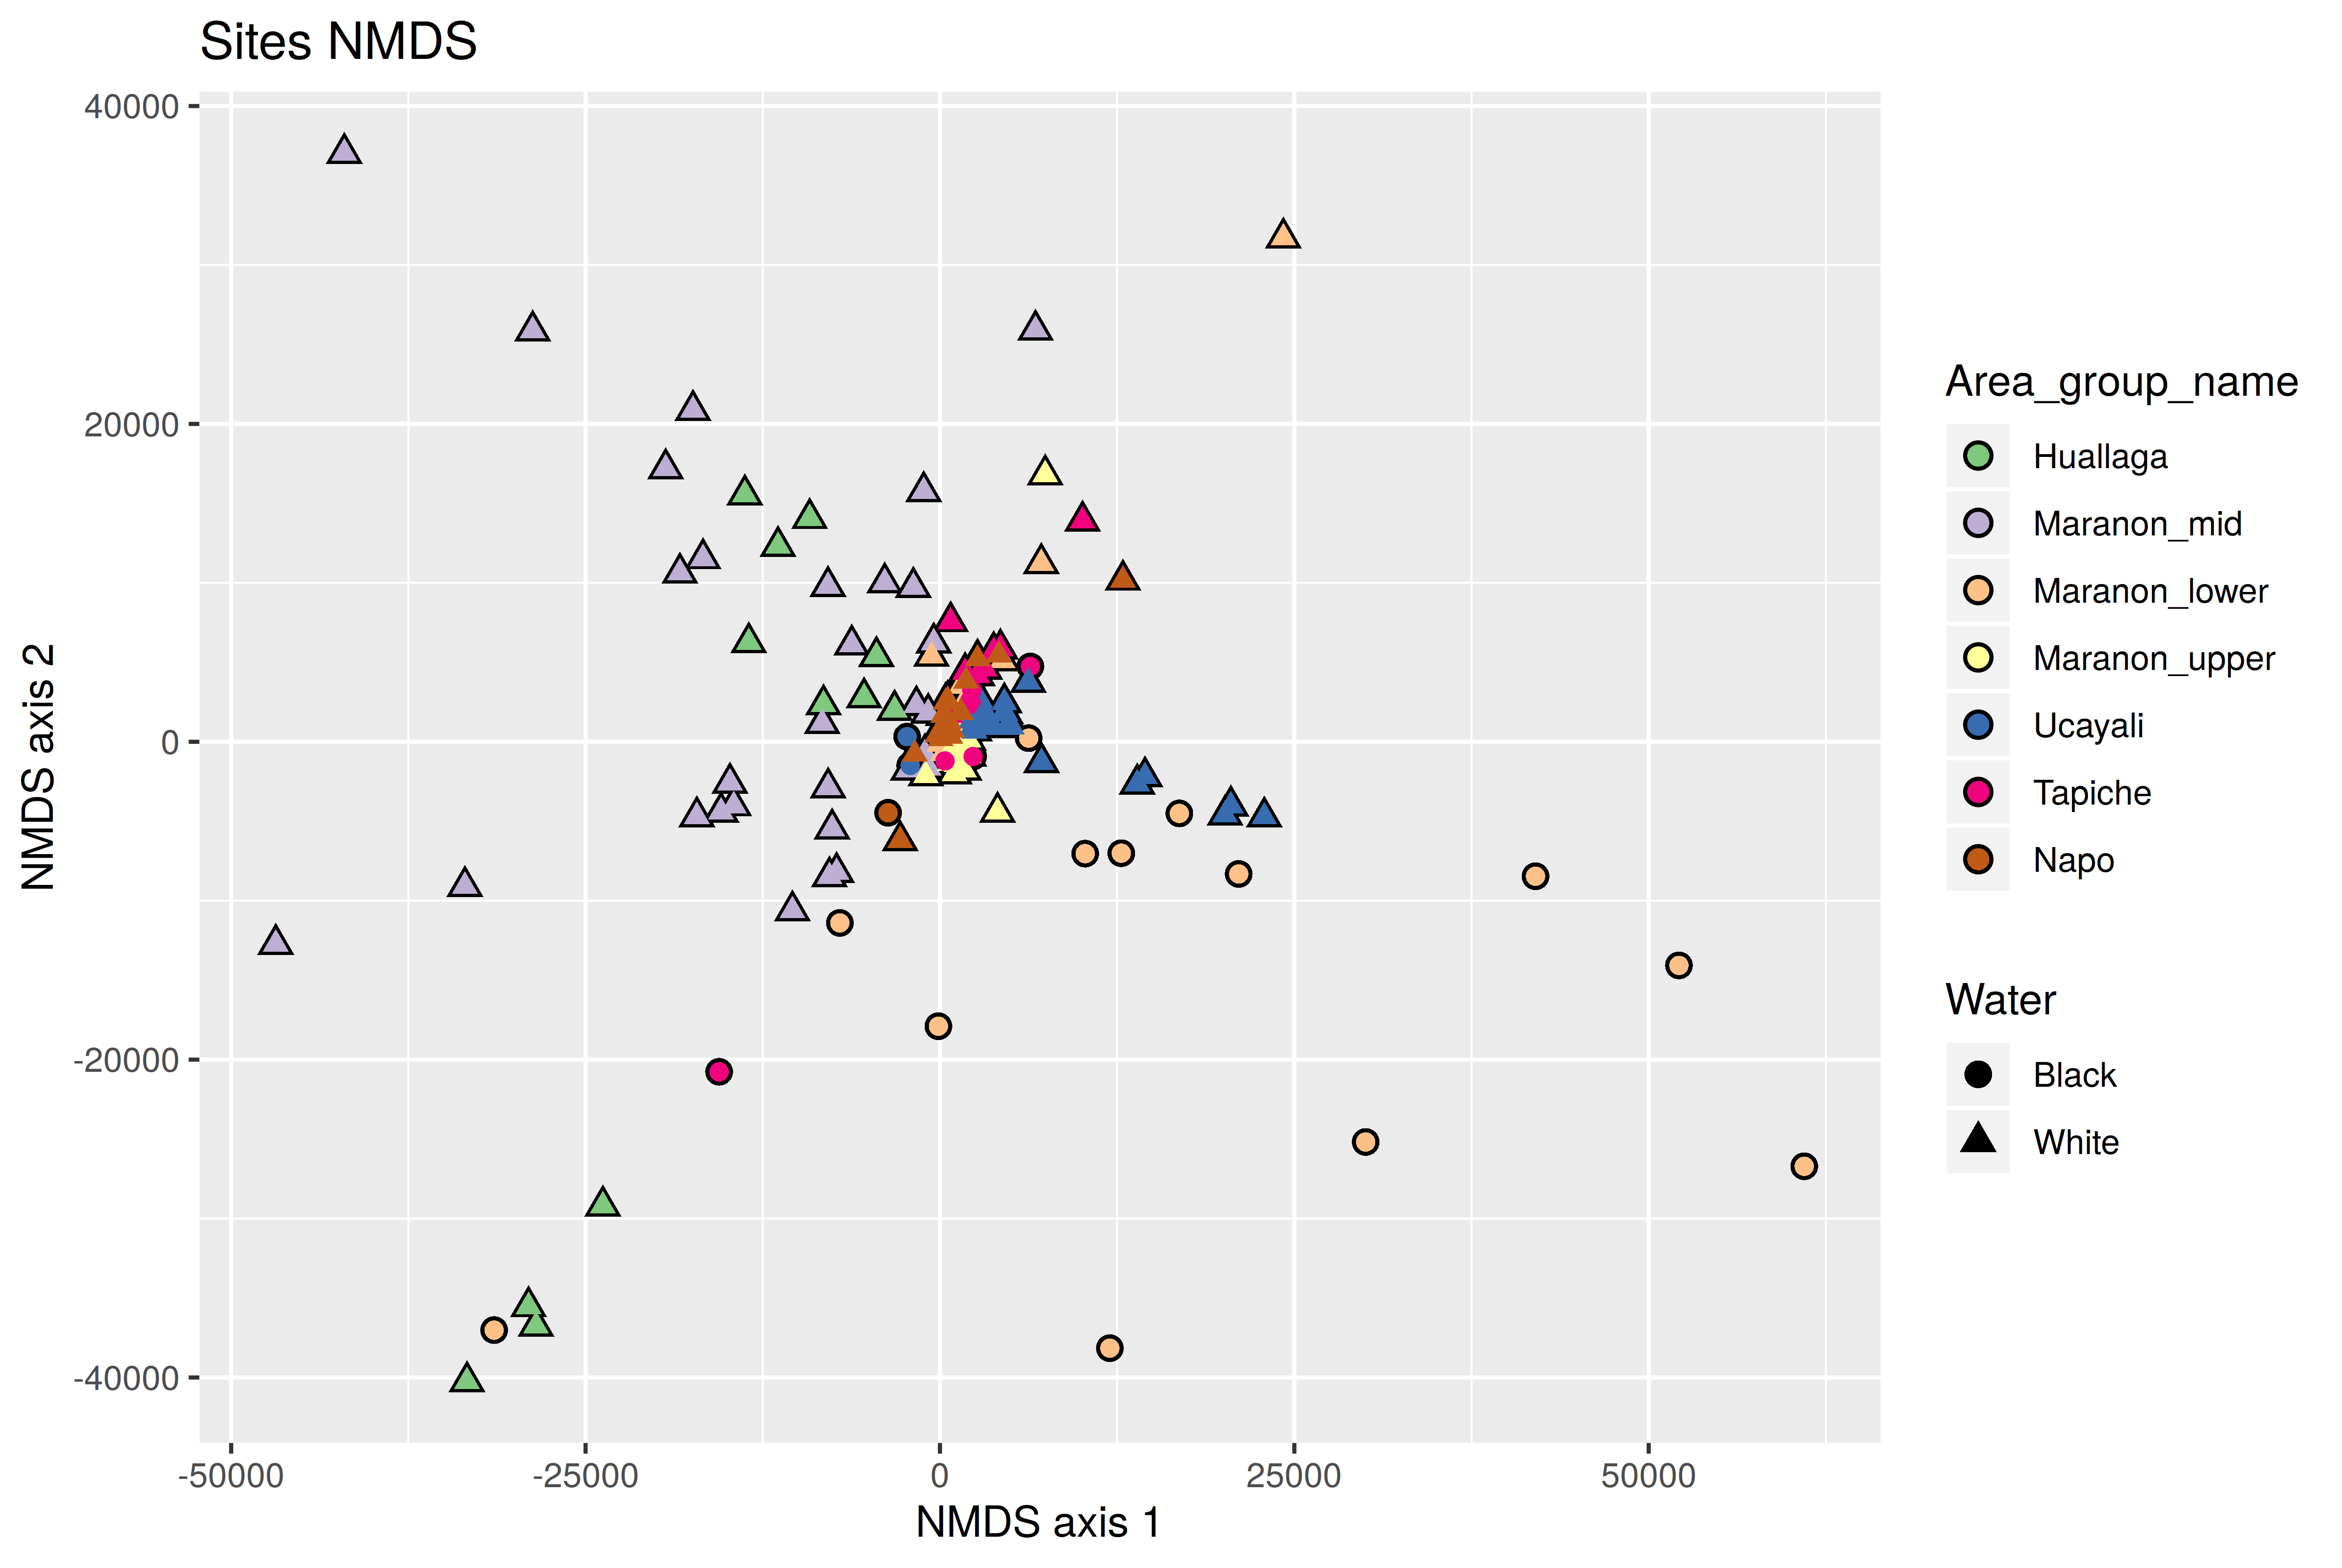
\includegraphics[width=\textwidth]{nmdsotu12euc}
		\caption{}
		\label{fig:nmdseuc}
	\end{subfigure}
\caption{NMDS ordination plots using Bray-Curtis \ref{fig:nmds} and Euclidean \ref{fig:nmdseuc} measure for dissimilarities. Bray-Curtis separates the rivers and colour much better than the Euclidean measure.}
\end{figure} 
%%The statistical question of goodness of fit is treated
%separately, not as an integral part of the procedure. 


\section{Permutational multivariate analysis of variance
}
\label{sec:permanova}

Permutational multivariate analysis of variance is a hypothesis testing technique that involves permuting the data set such that normality assumptions are avoided. Its use in ecology is to test if the OTU (read counts) distribution of two (or more) groups of samples is significantly different. Distance measures are used to define the relationships between the samples.

Particularly, the null hypothesis is: The centroids and dispersion of the groups, defined by a distance measure, are equivalent for all groups.
A rejection of the null means that the centroid and/or the dispersion is different between groups.

In the case of a one-way test, testing for the effect of a single grouping variable (our case), with $a$ groups and $n$ samples, we construct the distance matrix $D_{ij}$ using any measure relevant to our data. The matrix is constructed in the same way as in section \ref{sec:ordination} and it quantifies the dissimilarity between observations $i$ and $j$. The index of samples in each group $k$ is given by $I_{k}$. We are interested in testing if the grouping of samples by water colour produces significantly different distributions is OTU abundance.

Some statistics first need to be calculated, so that the test-statistic can be constructed. The total sum of squares is 
\begin{equation}
	SS_T = \frac{1}{n}\sum_{i<j} D_{ij}^2,
\end{equation}
where the sum is taken over the lower triangular distance matrix, excluding the diagonal. The group $k$ sums of squares is given by
\begin{align}
	SS_{w,k} &=\frac{1}{n_k} \sum_{i<j} \epsilon_{ij} D_{ij}^2 \\
	\epsilon_{ij} &=
	 \begin{cases}
	1, & \text{if}\ i,j \in I_{k} \\
	0, & \text{otherwise}
	\end{cases},
\end{align}
where the sum is taken over the samples belonging to the particular group. This amounts to summing up all the entries in the squared distance matrix that belong to group $k$. Summing up the group sums gives us the within groups sum-of-squares
\begin{equation}
	SS_w = SS_{w,white} + SS_{w,black}.
\end{equation}

With this we can define the among-group sum-of-squares $SS_A = SS_T - SS_w$ which can be used to construct a pseudo $F$-ratio
\begin{equation}
F=	\frac{SS_A/(a-1)}{SS_w (n-a)}, 
\end{equation}
where $(a-1)$ are the degrees of freedom associated with the grouping factor and $(N-a)$ are the residual degrees of freedom \cite{anderson_permutational_2005}. 

The distribution of this $F$-ratio under the null hypothesis is unknown, and we do not want to assume any. That is why permutations of the samples are used to generate a distribution of $F$. If the groupings have no discernible effect on the samples, then it is equally likely that the group labels were associated with any of the samples. So, under a true null hypothesis, we can shuffle the labels onto the samples, calculate $F$-ratios (denoted by $F_p$) and construct an empirical (discrete) distribution $\{F_p\}_p$.

If the null hypothesis is true, then the $F$-ratio calculated using the original ordering of labels relative to the samples will be similar to the values obtained under permutation. If the grouping however, produces a significant effect, then the original $F$ value will be larger than those obtained from the permutation $\{F_p\}_p$. To test for significance we calculate the probability associated with $F$ under the true null by counting the number of permuted ratios $F_p$ that have larger value than $F$ and dividing by the total number of permutations
\begin{equation}
	P = \frac{\#\{F_q\in\{F_p\}_p| F_q \geq F \}+1}{\#\{F_p\}_p+1}.
\end{equation}  
We include the original $F$ value in the distribution as well, that is why $+1$ is included in both denominator and numerator.


Not all possible permutations of the labels are necessary, a subset of them is enough to calculate a valid P-value. If it is calculated to be less than $5\%$ then we can reject the null. Of course the permutation affects greatly the calculated value so it is important that an appropriate scheme is used. The one we choose involves permuting the labels within sites. As explained earlier,  4-6 samples were collected for each site along the rivers. This means that even if samples collected close together came from different water colour, their dissimilarity would be relatively low when compared to far away sites. Thus, this shuffling will make it less probable for water colour to have a significant effect. 

The P-value calculated when using the OTU table and the permutation scheme outlined previously, with 2000 permutations, was $2.6\%$. When no restriction is put on the shuffling, the P-value is $0.05\%$, significantly smaller. This means the null hypothesis is rejected, and the two distributions have different centroids and/or dispersion, defined by the distance matrix. This is of course evident when one looks at the ordination plots in section \ref{sec:ordination}, which show a different spread of black and white water samples. This is especially true for NMDS.

The test was performed using the function adonis from the Vegan package in R.
\section{Classification Models}
\label{sec:classification}
\subsection{Logistic Regression}
\subsubsection{Bayesian approach}
Binary classification involves deciding in which of two groups (classes) an object (point) should be categorised. A point is constituted of a response variable and features. The purpose of a classifier is then to correctly identify the response variable given it's features and any other relevant information. 

Our data set's response variable is the water colour of the sample, defined here as $y_i \in \{ 1 (White),0 (Black)\}$ for the $i$th sample, where $i=1,...,N$. The notation $ \mathbf{x}_i = [x_{i1},x_{i2},...,x_{im}]$ is used to represent the $m$ dimensional row vector of features for the $i$th sample. Stacking up the feature vectors we construct the matrix $X_{ij}$, with rows denoting the samples and columns the features.

Assuming we do not know the response variable of a point we would like to calculate its probability of belonging to one of the classes  given its features
\begin{equation}
	P(y_i = 1(\text{White})| \mathbf{x}_i).
\end{equation}  
We can use Bayes' theorem to expand this probability into
\begin{equation}
	P(y_i =1| \mathbf{x}_i) = \frac{P( \mathbf{x}_i|y_i)P(y_i)}{P( \mathbf{x}_i)},
\end{equation}
 where the likelihood is given by $P(x_i|y_i)$, the prior by $P(y_i)$, and the marginal likelihood by $P(y_i)$. The prior indicates the point's probability of being in a class without taking into account its features. All the information about the point's features is encoded in the likelihood, where the probability of obtaining them is conditioned on the class. Finally, the marginal is the probability of obtaining the data, whatever the class of the point. 
 It can thus  be obtained by integrating out the class variable
 \begin{equation}
 	P( \mathbf{x}_i) = \sum_{y_i =0}^{1} P( \mathbf{x}_i|y_i)P( y_i).
 \end{equation} 

To decide in which class a point belongs to, we construct a decision boundary using the discriminant function
\begin{equation}
f( \mathbf{x}_i)=\log \frac{P(y_i=1 |  \mathbf{x}_i)}{P(y_i = 0 |  \mathbf{x}_i)}.
\label{eq:discr}
\end{equation}
If the function is greater than $0$ that means that the probability of the point coming from White water is greater than from Black water. 


We can adopt either a generative or a discriminative approach. The generative approach requires modelling the class conditional distributions $P(\mathbf{x}_i|y_i = 1)$ and $P(\mathbf{x}_i|y_i = 0)$, and using Bayes' theorem to obtain the discriminant function directly. Typical samples could also be generated by drawing data from $P(\mathbf{x}_i|y_i)$. The discriminant approach involves modelling the discriminant function \eqref{eq:discr} directly, using a linear model for example. We will be using the discriminative approach so as to avoid modelling the complex interaction between water colour and OTU-derived features.


A linear function (in parameters) can be used to model \eqref{eq:discr}. The features can be transformed by a non-linear function $\phi( \mathbf{x}_i) = [\phi_1( \mathbf{x}_i),\phi_2( \mathbf{x}_i),...,\phi_D( \mathbf{x}_i)]$ which can span a higher or lower dimensional space. The model is given by
\begin{equation}
	a = \log \frac{P(y_i=1 |  \mathbf{x}_i)}{P(y_i = 0 |  \mathbf{x}_i)} = \phi( \mathbf{x}) \bm{\theta}^T
\end{equation}
  where $ \bm{\theta} = [\theta_1,\theta_2,...,\theta_D]$ are the model parameters.
  
  We can simplify this expression by making the observation that the conditional class probabilities sum up to one
  \begin{align}
	\frac{P(y_i=1 |  \mathbf{x}_i)}{P(y_i = 0 |  \mathbf{x}_i)} &= \exp(a)\\
	\frac{P(y_i=1 |  \mathbf{x}_i)}{1-P(y_i=1 |  \mathbf{x}_i)} &= \exp(a)\\
	P(y_i=1 |  \mathbf{x}_i) &= \frac{\exp(a)}{1+\exp(a)},
  \end{align}
  and making use of the sigmoid function. The probability of point $i$ belonging to class $y_i \in \{1,0\}$  is thus
    \begin{align}
  	P(C = y_i |  \mathbf{x}_i, \bm{\theta}) &= P(C=1 |  \mathbf{x}_i)^{y_i}(1-P(C=1 |  \mathbf{x}_i))^{1-y_i}\nonumber\\
	&= \left(\frac{\exp(\phi( \mathbf{x}) \bm{\theta}^T)}{1+\exp(\phi( \mathbf{x}) \bm{\theta}^T)}\right)^{y_i}\left(\frac{1}{1+\exp(\phi( \mathbf{x}) \bm{\theta}^T)}\right)^{1-y_i} \nonumber\\
	&=\frac{\exp(\phi( \mathbf{x}) \bm{\theta}^T)^{y_i}}{1+\exp(\phi( \mathbf{x}) \bm{\theta}^T)}. \label{eq:singlelikelihood}
  \end{align}

%The likelihood has thus a Bernoulli distribution with success probability $P(y_i = 1| \mathbf{x}_i, \bm{\theta})$ being modelled as a function of the features.
%\begin{align}
%	P(y_i | \mathbf{x}_i  \bm{\theta}) &= \mu( \bm{\theta})^{y_i}(1 - \mu( \bm{\theta}))^{1-y_i}\\
%	\mu( \bm{\theta}) &= 	P(y_i =1 | \mathbf{x}_i  \bm{\theta}) \\
%	&= \sigma(\phi( \mathbf{x}) \bm{\theta}^T) = \frac{\exp(\phi( \mathbf{x}) \bm{\theta}^T)}{1+\exp(\phi( \mathbf{x}) \bm{\theta}^T)}.
%\end{align}
  
  
  The aim now is to figure out which distribution of parameters $ \bm{\theta}^T$ model a decision function best so that it classifies the most points correctly. To do that, we agglomerate all of our samples into two sets; train and test. The train set will be used to `learn' the best parameters and the test set to evaluate it's performance on unseen data. Thus the response variables $\mathbf{y}$ are grouped into $ \mathbf{y}_{train}$ and $ \mathbf{y}_{test} $, and the features $X$ into ${X}_{train}$ and $X_{test}$. The index set of samples belonging to train and test is given by $I_{train}$ and $I_{test}$ respectively.
  
  Because of the non-trivial interactions between our samples, we will be assuming that they are independent and identically distributed
  \begin{align}
   P(\mathbf{y} | X, \bm{\theta}) &=\prod_{n=1}^{N} P\left(C=y_{i} | \mathbf{x}_{n}, \bm{\theta}\right) \\ 
   &=\prod_{n=1}^{N} \frac{\exp \left(\phi\left(\mathbf{x}_{i}\right)\bm{\theta}^{T} \right)^{y_{n}}}{1+\exp \left(\phi\left(\mathbf{x}_{i}\right) \bm{\theta}^{T} \right)} .
   \label{eq:likelihood}
   \end{align}
	
	We can thus construct the posterior distribution of the parameters $\bm{\theta}$ by utilising Bayes' theorem and conditioning on the train sets
	\begin{align}
	P\left(\bm{\theta}|X_{train},\mathbf{y}_{train},s\right) = \frac{	P\left(\mathbf{y}_{train}|\bm{\theta},X_{train}\right) P\left(\bm{\theta}|s\right)}{P\left(\mathbf{y}_{train}|X_{train},s\right)}.
	\end{align}
   The $s$ denotes the (hyper)parameters of the prior that we have to assign from before hand. 
   The marginal likelihood is obtained by integrating out the parameters from the likelihood and the prior using the law of total probability
   \begin{align}
   P\left(\mathbf{y}_{train}|X_{train},s\right) = \int P\left(\mathbf{y}_{train}|\bm{\theta},X_{train}\right) P\left(\bm{\theta}|s\right) d\bm{\theta}.
   \end{align}
   The integral is usually intractable analytically because the parameters span a high-dimensional space.
   
   Once we have the posterior distribution we can use it on a new data set (test set), make predictions, and evaluate the model's performance using the predictive posterior distribution. This is done using the law of total probability 
   \begin{align}
		P({C} = 1|X_{train},\mathbf{y}_{train},\mathbf{x}_{i,test},s) &= \int P(C=1|\mathbf{x}_{i,test},\bm{\theta})P(\bm{\theta}|X_{train},\mathbf{y}_{train},s) d\bm{\theta}\label{eq:classprob} \\
		&= E(P(C=1|\mathbf{x}_{i,test},\bm{\theta})|X_{train},\mathbf{y}_{train},s),
   \end{align}
   where $\mathbf{x}_{i,test}=\mathbf{x}_{i \in I_{test}} $ is the features vector of any sample in the test set.  This is the probability of observation $i$ being in group 1 (White water) given the train data sets and the parameter of the prior. The probability $P(C=1|\mathbf{x}_{i,test},\bm{\theta})$ is the likelihood we encountered earlier and has the analytic form \eqref{eq:singlelikelihood}. Note that the distribution over the Class is not dependent on the parameters $\bm{\theta}$ since we integrated them out.
   
   
%   We only get a single value from posterior predictive probability. The power of Bayesian inference is that we can get a distribution over the parameter of interest. 
   
   A Bayesian approach to train and predict with such a model is to use Markov chain Monte Carlo (MCMC) methods to sample from the posterior and then approximate the posterior predictive probability \eqref{eq:classprob} using a Monte Carlo estimator. The $M$ samples obtained are denoted with $z^{(j)}$ and have the same dimension as the parameters $\bm{\theta}$. The estimate,
   \begin{align}
   	\int P(C=1|\mathbf{x}_{i,test},\bm{\theta}) P(\bm{\theta}|X_{train},\mathbf{y}_{train},s) d\bm{\theta} &= \frac{1}{M}\sum_{j=1}^M P(C=1|\mathbf{x}_{i,test},z^{(j)}) \\
   	&= \frac{1}{M}\sum_{j=1}^M  \frac{\exp(\phi(\mathbf{x}_{i,test}) \cdot(z^{(j)})^T)}{1+\exp(\phi( \mathbf{x}_{i,test}) \cdot z^{(j)}T)},
   \end{align} 
   can be evaluated with the generated samples for each point in the test set.
   
   
   The idea of MCMC is to generate samples $z^{(i)}$ while exploring the state space of interest (the space on which the posterior is defined, $\Theta$) using a markov chain mechanism. The chain is constructed such that it spends more time in more important regions. In particular, the aim is for the samples generated to mimic samples drawn from the target distribution ($P(\bm{\theta}|X_{train},\mathbf{y}_{train},s)$).
   The reason MCMC methods are of interest in our case is that they allow drawing samples from the target distribution if it can be evaluated up to a normalising constant (but does not have to be normalised, so we avoid calculating the marginal likelihood). 
   
   The $M$ resulting samples can be used to approximate the target density 
   \begin{align}
   	P_M(\bm{\theta}|X_{train},\mathbf{y}_{train},s) = \frac{1}{M}\sum_{i = 1}^M \delta(\bm{\theta} = z^{(i)}),
   \end{align}
   where $\delta(\bm{\theta} = z^{(i)})$ denotes the Dirac delta function centred at the vector $z^{(i)}$. Using this point-mass function, integrals $I(f)$ can be approximated with sums $I_M(f)$ that converge in the following manner
   \begin{equation}
   	I_M(f) = \frac{1}{M}\sum_{i = 1}^M f(z^{(i)})     \underset{M \rightarrow \infty}{{\rightarrow}} \int_{\Theta} f(\theta)P_M(\bm{\theta}|X_{train},\mathbf{y}_{train},s) d\theta = I(f).
   	\label{eq:convergencemcmc}
   \end{equation}
   If the $z_{(i)}$ samples were i.i.d, the estimator $I_M(f)$ is unbiased and by the strong law of large numbers it almost surely converges to $I(f)$. MCMC samples need to satisfy some conditions for them to be used in monte carlo estimates.
   
   The ergodic theorem generalises the law of large numbers. Suppose that $\{z^{(i)}\}_{i \in \mathrm{N}}$ is an ergodic Markov Chain with stationary distribution our target distribution and function $f:\mathrm{R}^D \rightarrow \mathrm{R}$ defined on the state space of our sample. Then \eqref{eq:convergencemcmc} holds.
   
   This motivates the use of Metropolis-Hastings, an MCMC sampling method. A step of the algorithm involves drawing a sample $z^*$ from a proposal distribution (that aims at exploring the state space) $q(z^*|z^{(i-1)})$ given the current value of the chain $z^{(i-1)}$. Then the chain moves to the candidate value $z^*$ with an acceptance probability 
   \begin{equation}
   	min\left( 1,\frac{p(z^*)q(z^*|z^{(i-1)})}{p(z^{(i-1)})q(z^{(i-1)}|z^*)}\right),
   \end{equation} 
   where $p(z)$ is the unnormalised target density (or the target density up to a constant, the marginal likelihood, independent of $z$).
   
   If the candidate $z^*$ is not accepted then a new one is drawn from the proposal conditioned on the previously accepted sample. The process goes on up until we have generated a sufficient number of samples. More detailed explanation of the algorithm and the theory behind Markov Chain can be found in \cite{lange_markov_2010}.
   %ADD PROBABILITY NOTES IF TIME
   
	Instead of using Metropolis-Hastings (MH), Hamiltonian Monte Carlo (HMC) was used. When compared to a MH using a Gaussian random-walk as proposal distribution, it reduces the correlation between successive sampled states, and thus it needs fewer samples to approximate integrals. An outline of the method is given in section \ref{section:hmc}.
	
	
	
   
%   
%   We will hence outline some basic theory of Markov Chains so that the samplers subsequently discussed are coherent to the reader. This will not be an formal treatment on the subject, and no proofs to theorems or corollaries will be given. More extensive material on the subject can be found elsewhere .
%   
%   We introduce Discrete time and space Markov Chains because of the ease of pressentation. Let $z^0,z^1,...$ be a sequence of random variables, each of which takes some value in a state space $E \subseteq \mathrm{Z}$. We denote $\mathrm{N}_0 = \mathrm{N} \cup \{0\}$. 
%   \begin{defn}
%   	
%   \end{defn}
%   
%   The aim of MCMC is to construct a markov chain whose stationary distribution is the target distribution. 
%   
%   However, MCMC samples are not i.i.d and thus have different convergence rates. MCMC 

   
   
 %%%%%%%%%%%%%%%%%%%%%  
\subsubsection{Maximum Likelihood Estimation}

The Maximum Likelihood approach to fitting a logistic regression model to the data involves, as the name suggests, maximising the likelihood of response variables given the features and the parameters , with respect to the parameters \eqref{eq:likelihood}.

Instead of looking at the likelihood we can look at its log transform, which has the same order relations as the likelihood
\begin{equation}
	P(a_1|b) > P(a_2|b) \Leftrightarrow 	\log P(a_1|b) >\log P(a_2|b).
\end{equation} 
We can define the loss function by taking the negative logarithm of the likelihood, which gives what is called the cross-entropy loss function
\begin{align}
	L(\bm{\theta})= - \left(\sum_{n=1}^N y_n \phi\left(\mathbf{x}_{i}\right)\cdot\bm{\theta}^{T} -\log\left(1+\exp\left(\phi\left(\mathbf{x}_{i}\right)\bm{\theta}^{T}\right)\right) \right).
\end{align}
Thus, instead of maximising the likelihood, we can minimise the loss, which allows for more computational accuracy.  
The parameters $\bm{\theta}^*$ that minimise this loss are then used for the prediction of new features. If the discriminant function,
\begin{align}
	 \log \frac{P(C=1 |  \mathbf{x}_i)}{P(C = 0 |  \mathbf{x}_i)} = \phi( \mathbf{x}) (\bm{\theta}^*)^T,
\end{align}
 is bigger than 0 then the point is classified as coming from white water, and if it is smaller then from black. 
 
 Regularisation can also be introduced that would reduce over fitting on the training data. If not employed, the model might become too complicated, modelling the noise in our data, and thus not generalisable. Using regularisation in machine learning amounts to penalising model complexity by adding a term to the loss function. This will cause some of the parameters to shrink towards zero, thus creating a simpler model.
 
 Ridge, or $L_2$ regularisation, involves adding the $L_2$ norm of the parameters to the loss function
 \begin{equation}
 		L(\bm{\theta},s)= - \left(\sum_{n=1}^N y_n \phi\left(\mathbf{x}_{i}\right)\cdot\bm{\theta}^{T} -\left(1-y_n\right)\log\left(1+\exp\left(\phi\left(\mathbf{x}_{i}\right)\bm{\theta}^{T}\right)\right) \right) + s||\bm{\theta}||_2.
 \end{equation}
  A sparsity parameter $s$ is used to control how much the model complexity will be penalised. With Ridge the parameters are prevented from taking large values.
  
  Lasso, or $L_1$ regularisation, involves adding the $L_1$ norm of the parameters to the loss function
 \begin{equation}
L(\bm{\theta},s)= - \left(\sum_{n=1}^N y_n \phi\left(\mathbf{x}_{i}\right)\cdot\bm{\theta}^{T} -\log\left(1+\exp\left(\phi\left(\mathbf{x}_{i}\right)\bm{\theta}^{T}\right)\right) \right) + s||\bm{\theta}||_1.
\end{equation}
	Use of the $L_1$ norm allows some parameters to become zero during training, thus reducing the model's complexity. This is in contrast to Ridge which generally will not force any parameters to take a zero value, but something close to it.
	This ability of Lasso makes it also useful as a feature selection method, which is especially important in data sets with a large number of features. 
	However, Lasso tends to select only one feature from a group of highly correlated ones, even if they are all descriptive. For our data set, where linear relationships might arise accidentally and not bear ecological significance, this tendency of the algorithm might mask the contribution of otherwise significant species. 
	
	
	Furthermore, adding an $L_1$ norm to the loss function means it is not longer differentiable. Therefore, minimisation algorithms have to be employed to get the best parameters. 
	
	Choosing one of these regularisation techniques is equivalent to maximising the posterior distribution $P(\bm{\theta}|X_{train},\mathbf{y}_{train},s)$, and choosing an appropriate prior for the parameters. To demonstrate, let's assume that the prior is a multivariate normal distribution with mean zero and the identity matrix multiplied by a constant as covariance. Then the log posterior can be written as
	\begin{align}
		P(\bm{\theta}|s) &= (2\pi)^{-\frac{M}{2}}s^{-\frac{1}{2}}\exp\left(-\frac{\bm{\theta}\cdot\bm{\theta}^T}{2s}\right)\\
		\log P(\bm{\theta}|X_{train},\mathbf{y}_{train},s) &=\left(\sum_{n=1}^N y_n \phi\left(\mathbf{x}_{i}\right)\cdot\bm{\theta}^{T} -\log\left(1+\exp\left(\phi\left(\mathbf{x}_{i}\right)\bm{\theta}^{T}\right)\right) \right) - \frac{\bm{\theta}\cdot\bm{\theta}^T}{2s},
	\end{align}
  by ignoring constants, like the marginal likelihood $P(\mathbf{y}_{train}|X_{train},s)$ and the prior constants that do not depend on the parameters. Therefore, maximising the posterior with multivariate Normal prior is equivalent to minimising the loss with an $L_2$ regularisation. 
  
  
  Using instead independent Laplace priors centred at zero for each parameter
  \begin{align}
  		P(\bm{\theta}|s) &= \prod_{i = 1}^{M} \frac{1}{2s} \exp\left(\frac{|\theta_i|}{2s}\right),
  \end{align} 
  and maximising the posterior, is equivalent to minimising the loss with lasso regularisation.
  
  An advantage of the Bayesian method is that we get a distribution over the parameters instead of a single value estimate. This gives us a better idea of how important a feature is and how considerable the effect. A disadvantage is that it needs to sample a large number of values from the posterior to approximate it well. This is more so when the parameters' dimension is larger. Therefore, it is usually a significantly slower algorithm.
  
  The hyperparameters we cross-validated included the sparsity parameter $s$, the intercept, and a class balance term that gives more weight to the minority class in the loss function. 
  
  Linear regression was performed using the package scikit-learn in python \cite{scikit-learn}. The MCMC approach was carried out using PyMC3, a python package for Bayesian statistical modelling \cite{Salvatier2016}.
  
  
\subsection{Random Forest}
Random Forest is an ensemble method that works by training multiple decision trees and averaging their predicted class when it comes to classification. The combination of trees is done to reduce the overfitting of single decision trees on the train set \cite{hastie_elements_2009}. In particular, trees grown very deeply to learn complex patterns in the data have often low bias but very high variance. 

To combat this the features and observations used by each tree are randomly sub-sampled from the training set (with or without replacement) \footnote{Sampling only the observations with replacement is called bagging (bootstrap aggregating)}. Thus the random forest algorithm averages out deep decision trees trained on different parts of the training set, so as to reduce their variance.  

 \subsubsection{Decision Trees}

To illustrate how binary decision trees work, let's consider the classification of humans into male and female using two features: height in centimetres and weight in kilograms. An example of a decision tree applicable for such a problem is given in figure \ref{fig:extree}. The root node splits the features space of height into two regions, one above 180cm and one below. In the first region, the tree classifies all points as male. The second region is further split into two based on weight; above and below 80kg. 
\begin{figure}
\centering
	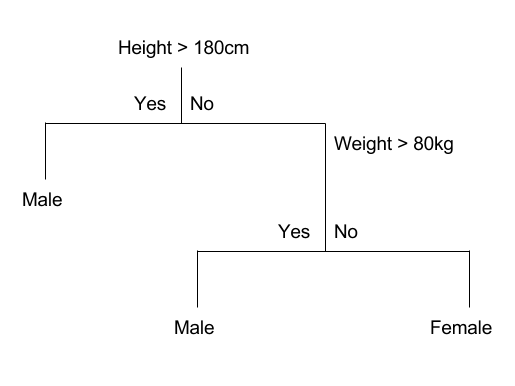
\includegraphics[width=0.5\textwidth]{Example-Decision-Tree}
	\caption{An example of a decision tree constructed for the classification to males and females}
	\label{fig:extree}
\end{figure}

Decision trees constructed by Random Forest are done so using the Classification and Regression Trees (CART) algorithm. These are binary trees were each node represents a single input feature and a split condition in that feature's space. The leaf nodes of the trees (end points) contain an output variable (class label). The selection of which features to be used at each node is done using a cost function. The construction of a tree ends when a predefined stopping condition is met.


Our data sets is made up of $N$ response variables $y_i \in \{1,0\}$ and features $\mathbf{x}_i \in \mathrm{R}^p$. Let's also define the regions our feature space is split into by each node of the tree by $R(j,s)$, where $j$ is the splitting feature and s is the split point. The pair of regions is given by 
\begin{equation}
	R_1(j,s) = \{X|X_j \leq s\} \text{ and } 	R_2(j,s) = \{X|X_j > s\}.  
\end{equation}

The proportion of class $k \in \{1,0\}$ observations in region $m$ which has a total of $N_m$ observations is given by
\begin{equation}
	\hat{p}_{m,k}(j,s) = \frac{1}{N_m} \sum_{\mathbf{x}_i \in R_m(j,s)} I(y_i = k), 
\end{equation}
where $I(y_i=k)$ is the indicator function (equals to one when $y_i =k$, zero otherwise) and the sum is over all the points which lie in region $R_m$. The proportion depends on the splitting feature and point $(j,s)$ of the region $R_m$.


To create a tree we need to divide up the feature space; a greedy approach called recursive binary splitting is used. It involves searching over all available features (to that node) and all split points to find the split (or regions) with the lowest cost.  To create this cost function, impurity measures are used, which quantify how pure a node is.
One commonly used  measure is the Gini index which takes the form
\begin{equation}
	G_m = 2\hat{p}_{m,1}(1-\hat{p}_{m,1}),
\end{equation}
in region $m$ for binary classification. When samples at a node (or region)  belong  with equal proportions to both classes (thus a bad/impure split), the index takes the value 0.5. When the node has samples in only one class it takes the value 0 (a perfect/pure split).

To construct the cost function we need to take into consideration the number of observations in the two child nodes $N_{mL},\ N_{mR}$ created by splitting the $m$ node, and weight the corresponding node impurity measure. This gives the cost function of node $m$ 
\begin{align}
	\Delta G_m &=G_m - G_{mL} \frac{N_{mL}}{N_m} - G_{mR}\frac{N_{mR}}{N_m}\\ &=2\hat{p}_{mL,1}(j,s)(1-\hat{p}_{mL,1})\frac{N_{mL}}{N_m} + 2\hat{p}_{mR,1}(1-\hat{p}_{mR,1})\frac{N_{mR}}{N_m},
	\label{eq:decreaseimpurity}
\end{align}
which depends on the choice of region $m$, and consequently on the split feature and point $(j,s)$. The subscripts $mL$ and $mR$ denote the two child nodes created after the split, and $\hat{p}_{mR,1}$ the proportion of samples in class 1 in the right node. This cost function is called `decrease in Gini impurity' at node $m$.

The feature (from those available to the tree) and split point that maximises the decrease in impurity $\Delta G_m$ are used to construct child nodes, increasing the depth of the tree.

The most common stopping criterion is to set a minimum number of observables that each node needs to satisfy before it is further split. If the count is less than that then the node becomes a leaf node.  

\subsubsection{Aggregating}
As mentioned earlier, trees used in random forest are not trained on the whole data set. In particular, bagging is usually employed so that each tree fits a model on a different set of observables. Furthermore, at each node of a tree, a predetermined number of features are sampled without replacement; only these are considered in the splitting condition. Usually this number is set to the square root of the total number of features in the train set (rounded up).

When it comes to prediction, the output class probability predicted by each tree $T_i(\mathbf{x})$ is averaged over all $B$ trees to give the class probability of the ensemble
\begin{align}
	T_i(\mathbf{x}_{test}) &= P(C=1|\mathbf{x}_{test})_i\\ &= \text{Proportion of class 1 observables in leaf node reached by }\mathbf{x}_{test}\\
	P(C = 1|\mathbf{x}_{test},\{T_i\}_{1}^B) &= \frac{1}{B} \sum_{i=1}^B T_i(\mathbf{x}_{test}) .
\end{align}

 The construction of the algorithm allows it to determine which features offer most of the explanatory power in separating samples. There are several ways to do this and none of them outperforms the other in all cases (since explanatory power is a difficult concept to define). One approach uses the out-of-bag samples that were not used in the construction of a tree (if bagging was used). Its prediction accuracy on these samples is measured and used as a benchmark for feature evaluation. Then the values for a feature in the out-of-bag data set are randomly permuted, and the prediction accuracy of the tree is tested again. The drop in accuracy is associated with the predictive power of the feature whose values where permuted. This is done for all features, and the loss in accuracy is averaged over all trees. The larger the drop, the more predictive the feature. 
 
 Another way is to measure the mean decrease in impurity of each feature. For a feature $X_j$ this is done by adding up the weighted decrease in impurity for all nodes where $X_j$ is used, and then average over all trees in the forest. The formula is given by 
 \begin{equation}
 	Importance(X_j) = \frac{1}{B} \sum_{b= 1}^{B}\sum_{t \in \phi_b} I(j_t =j)\left[prop(t)\Delta G_t\right],
 \end{equation}
where the sum is over all trees $b$ and all nodes of the tree $\phi_b$, and $I(j_t =j)$ is the indicator function that takes the value 1 when node $t$ is split using variable $X_j$. The proportion of samples, from the initial number, at node $t$ is given by $prop(t)$ \cite. \textbf{Gilles} 
%
% With just bagging, the algorithm produces an ensemble of structurally similar trees. That's why feature sampling is used in random forests; to reduce the correlation between trees.
 
 The random forest algorithm was implemented using scikit-learn in python. The gini impurity measure is used both for tree growing and for feature importance (using also trees' depth as an indicator). The number of trees, the stopping criterion and whether to bootstrap the observations were cross validated. 
%%%~~~~~~~~~~~~~~~~~~~~~~~~~~~~~~~~~~~~~~~~~~~~~~~~~~~~~~~~~~~~~~~~~
%% DATA SPLITTING
%%~~~~~~~~~~~~~~~~~~~~~~~~~~~~~~~~~~~~~~~~~~~~~~~~~~~~~~~~~~~~~~~~~
%\section{Data-Splitting}
%
%Together with the OTU table, our data also include the location of the samples in the rivers (in Easting and Northing coordinates) and in which part of the river they belong to. Because of this location attribute, our samples cannot be said to be independent. Thus, the way we choose to split our data into training and testing sets will surely affect the accuracy of the classifier. For example, testing on a set that is composed of samples maximally distant from the ones in the training set (see Figure \ref{fig:groupsamp}) will produce different results than testing on a set with all samples in close proximity to the ones in the training set (see Figure \ref{fig:stratsampl}).
%
%To avoid choosing a split method, several ones have been employed that represented different splitting conditions. The classifiers have then been tested on all of them so as to evaluate how well they can perform under various circumstances.
%%% Stratified an group folds for tain test split plot
%\begin{figure}[h]
%\centering
%\begin{subfigure}{0.4\textwidth}
%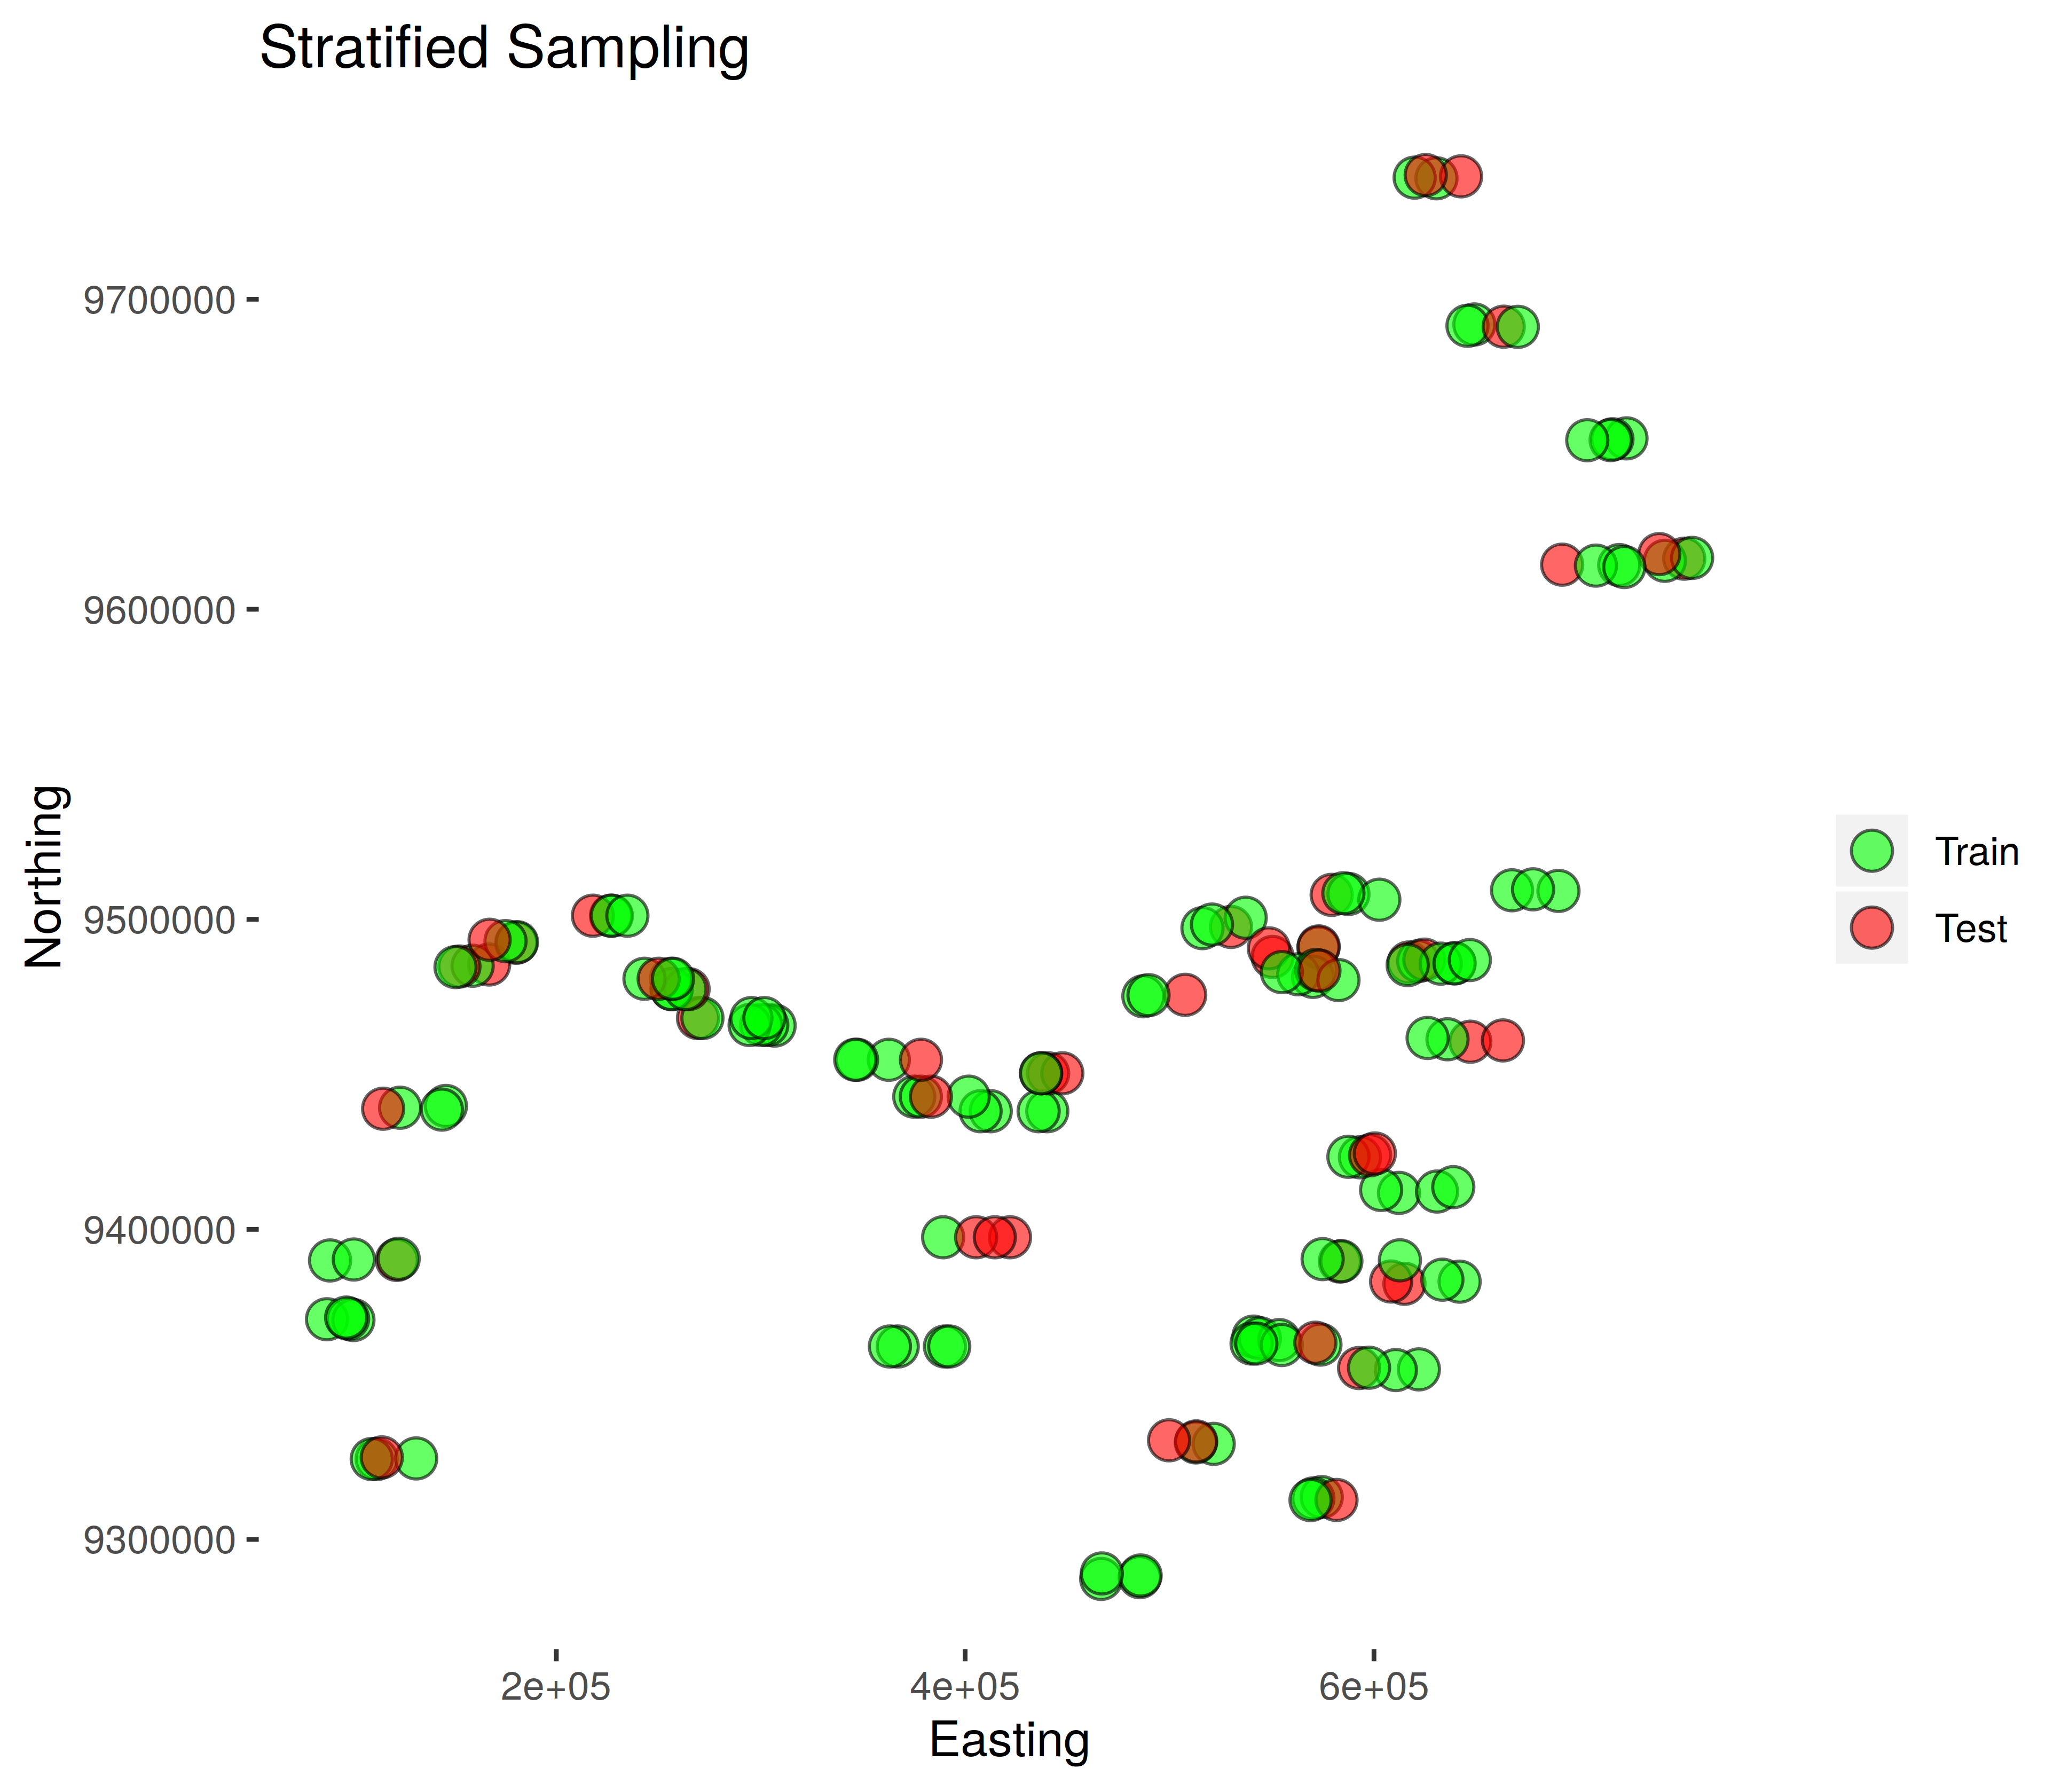
\includegraphics[width = \textwidth]{stratsamp.png}
%\end{subfigure}
%\begin{subfigure}{0.4\textwidth}
%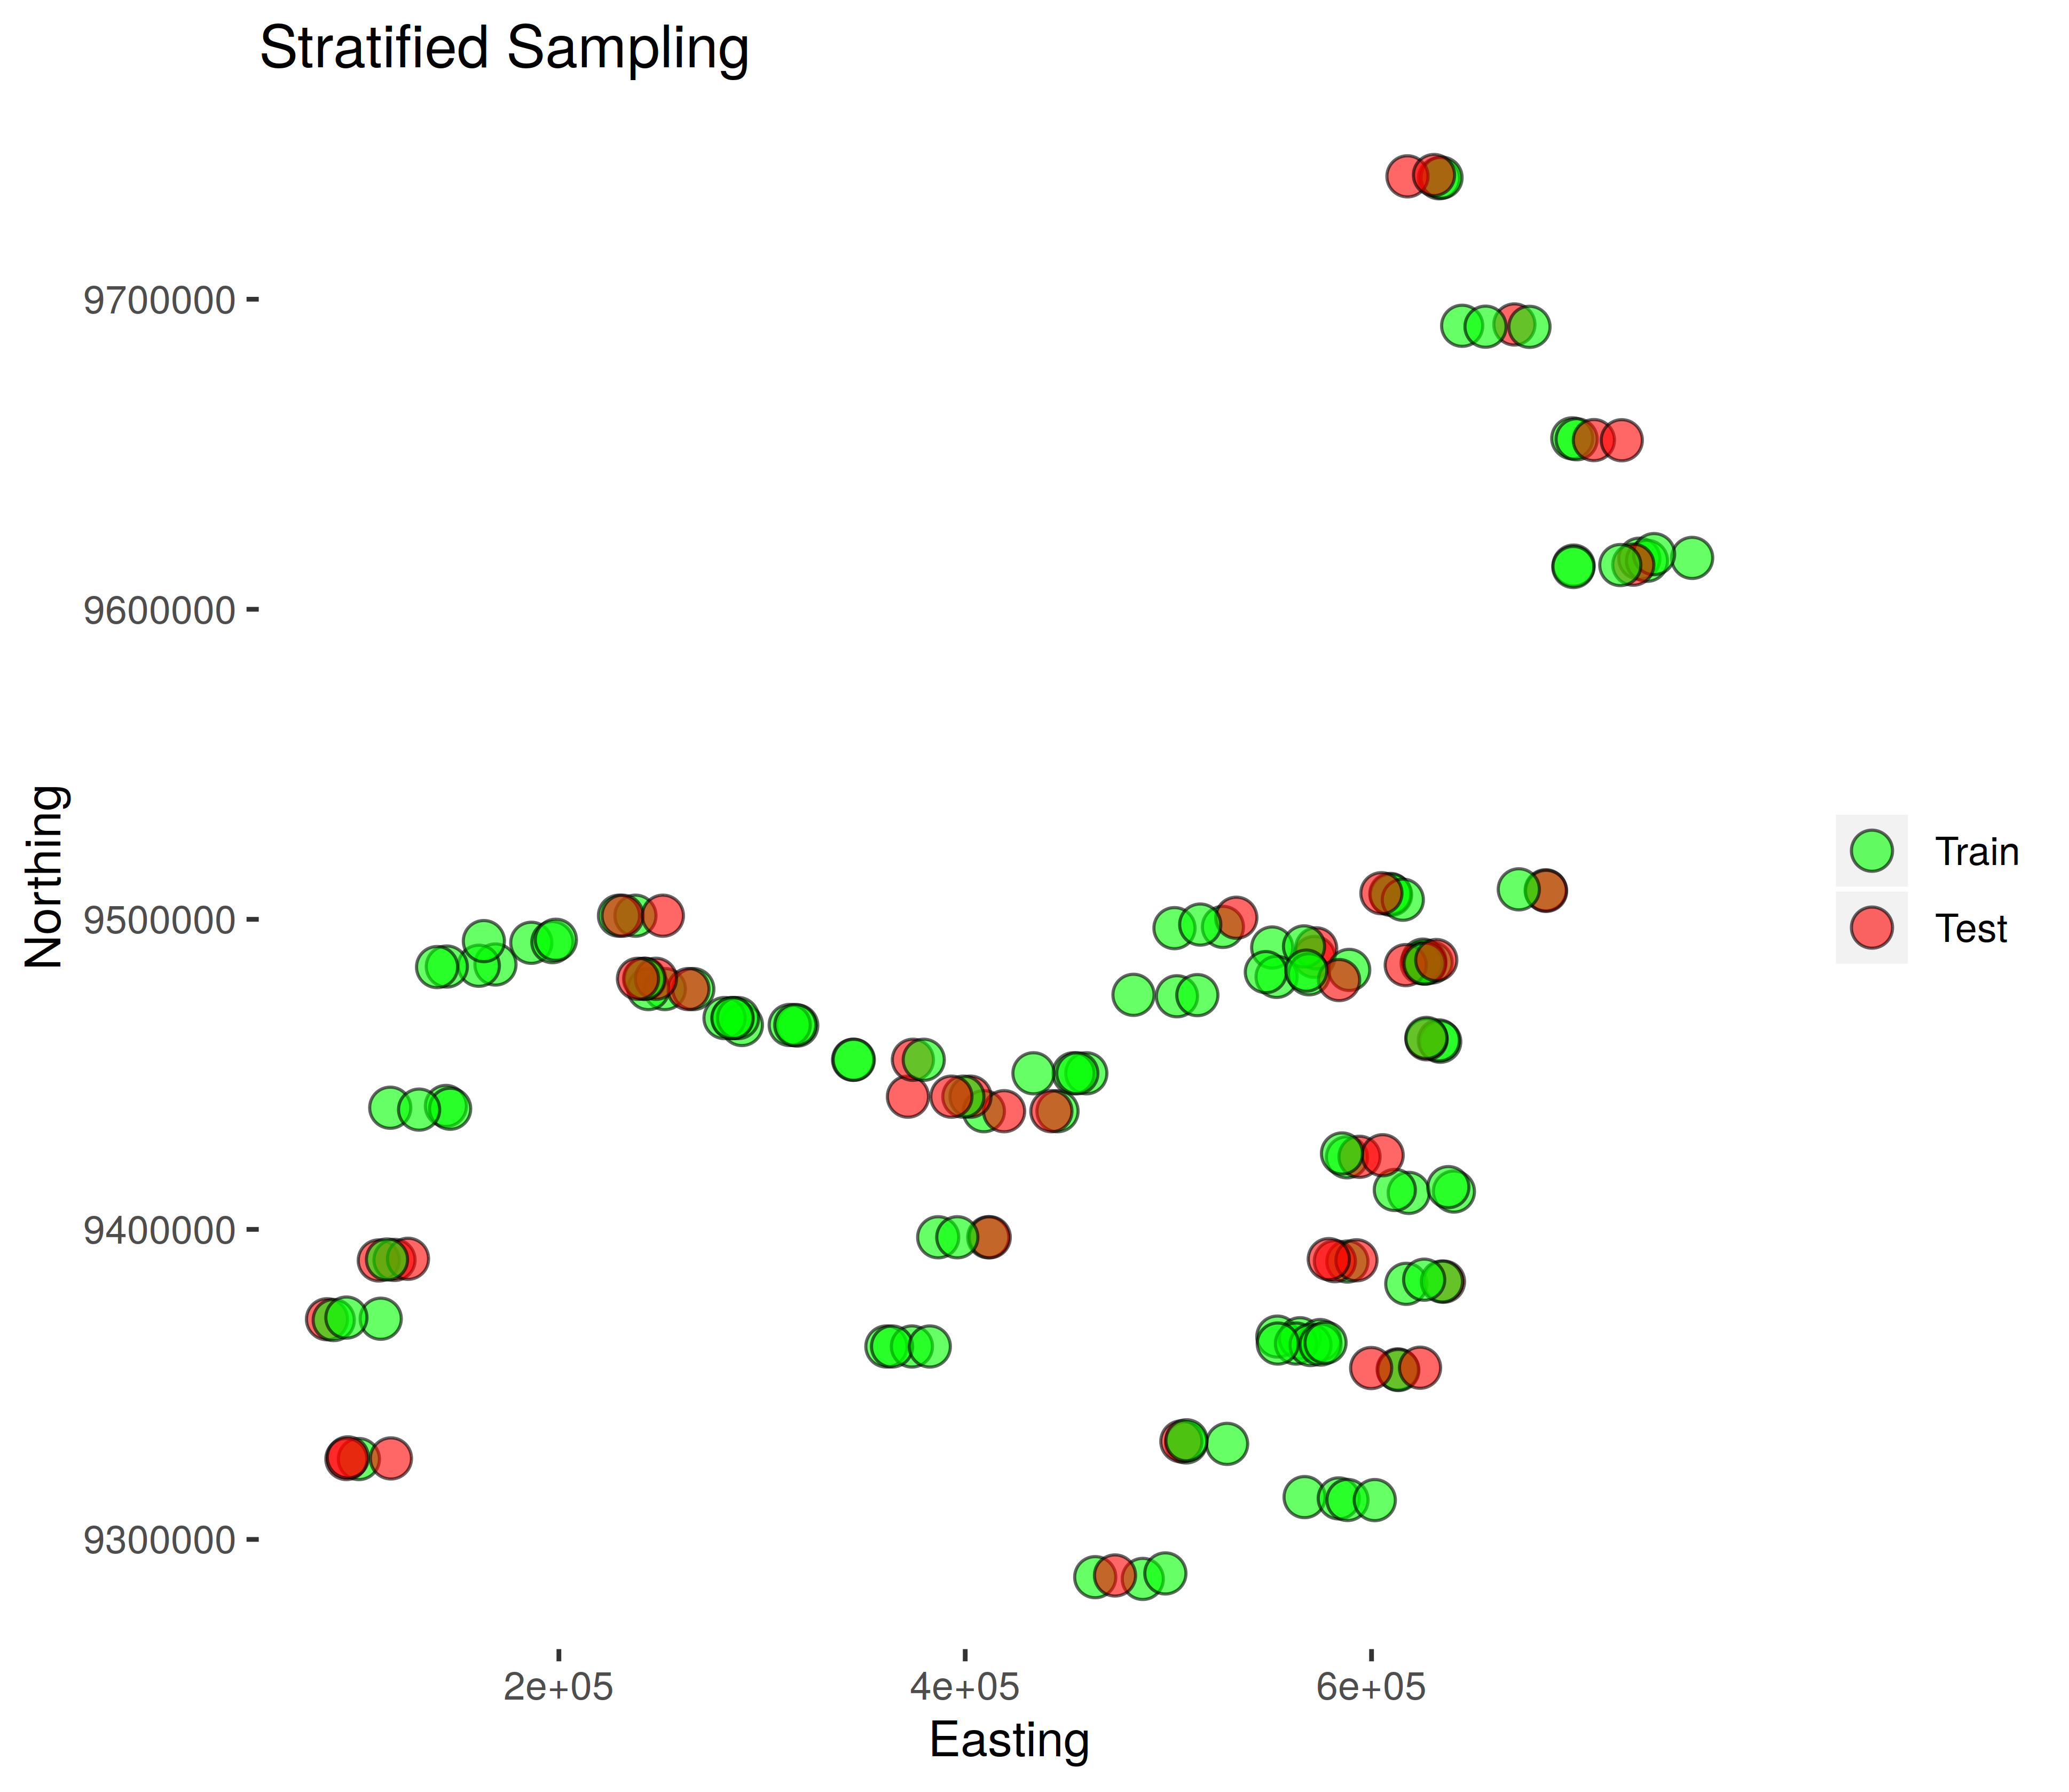
\includegraphics[width = \textwidth]{stratsamp2.png}
%\end{subfigure}
%\caption{Test set samples are geographically among Train set samples. This represents a maximally similar split which is created by ensuring constant distribution of samples in each part of the river in both the Train and Test set.}
%\label{fig:stratsampl}
%\end{figure}
%
%%Group sample plot
%\begin{figure}[h]
%\centering
%\begin{subfigure}{0.4\textwidth}
%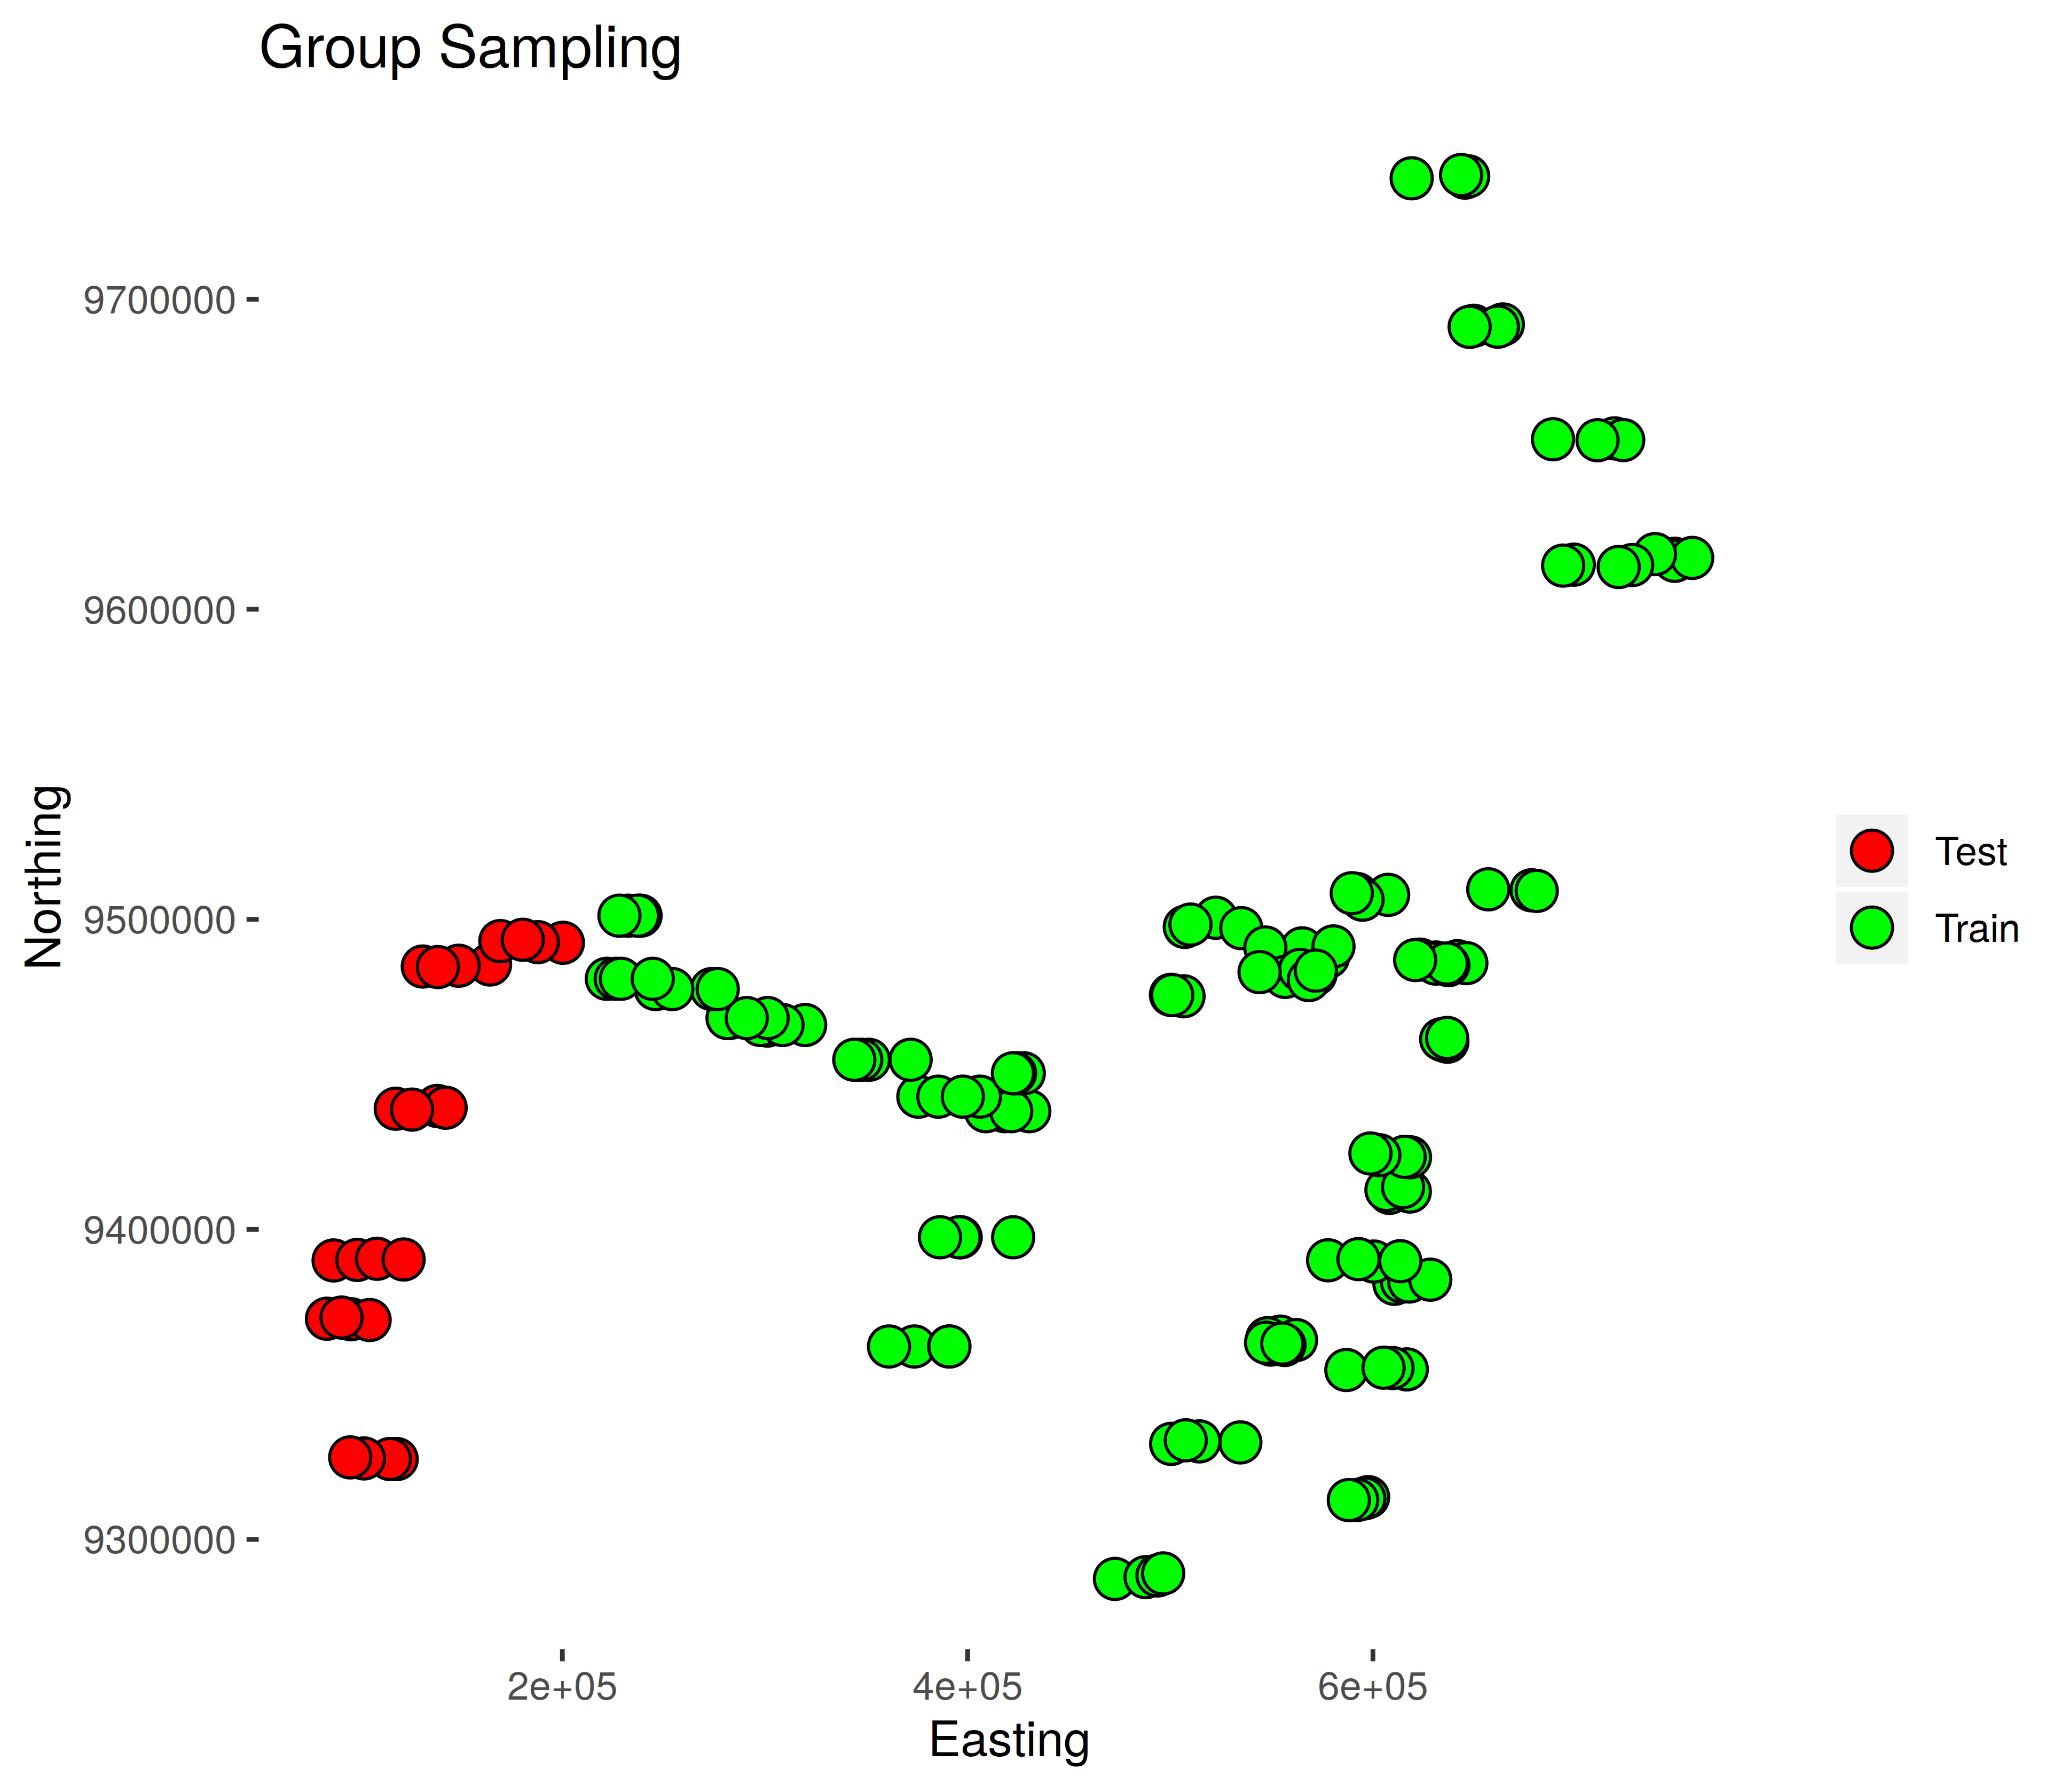
\includegraphics[width = \textwidth]{groupsamp.png}
%\end{subfigure}
%\begin{subfigure}{0.4\textwidth}
%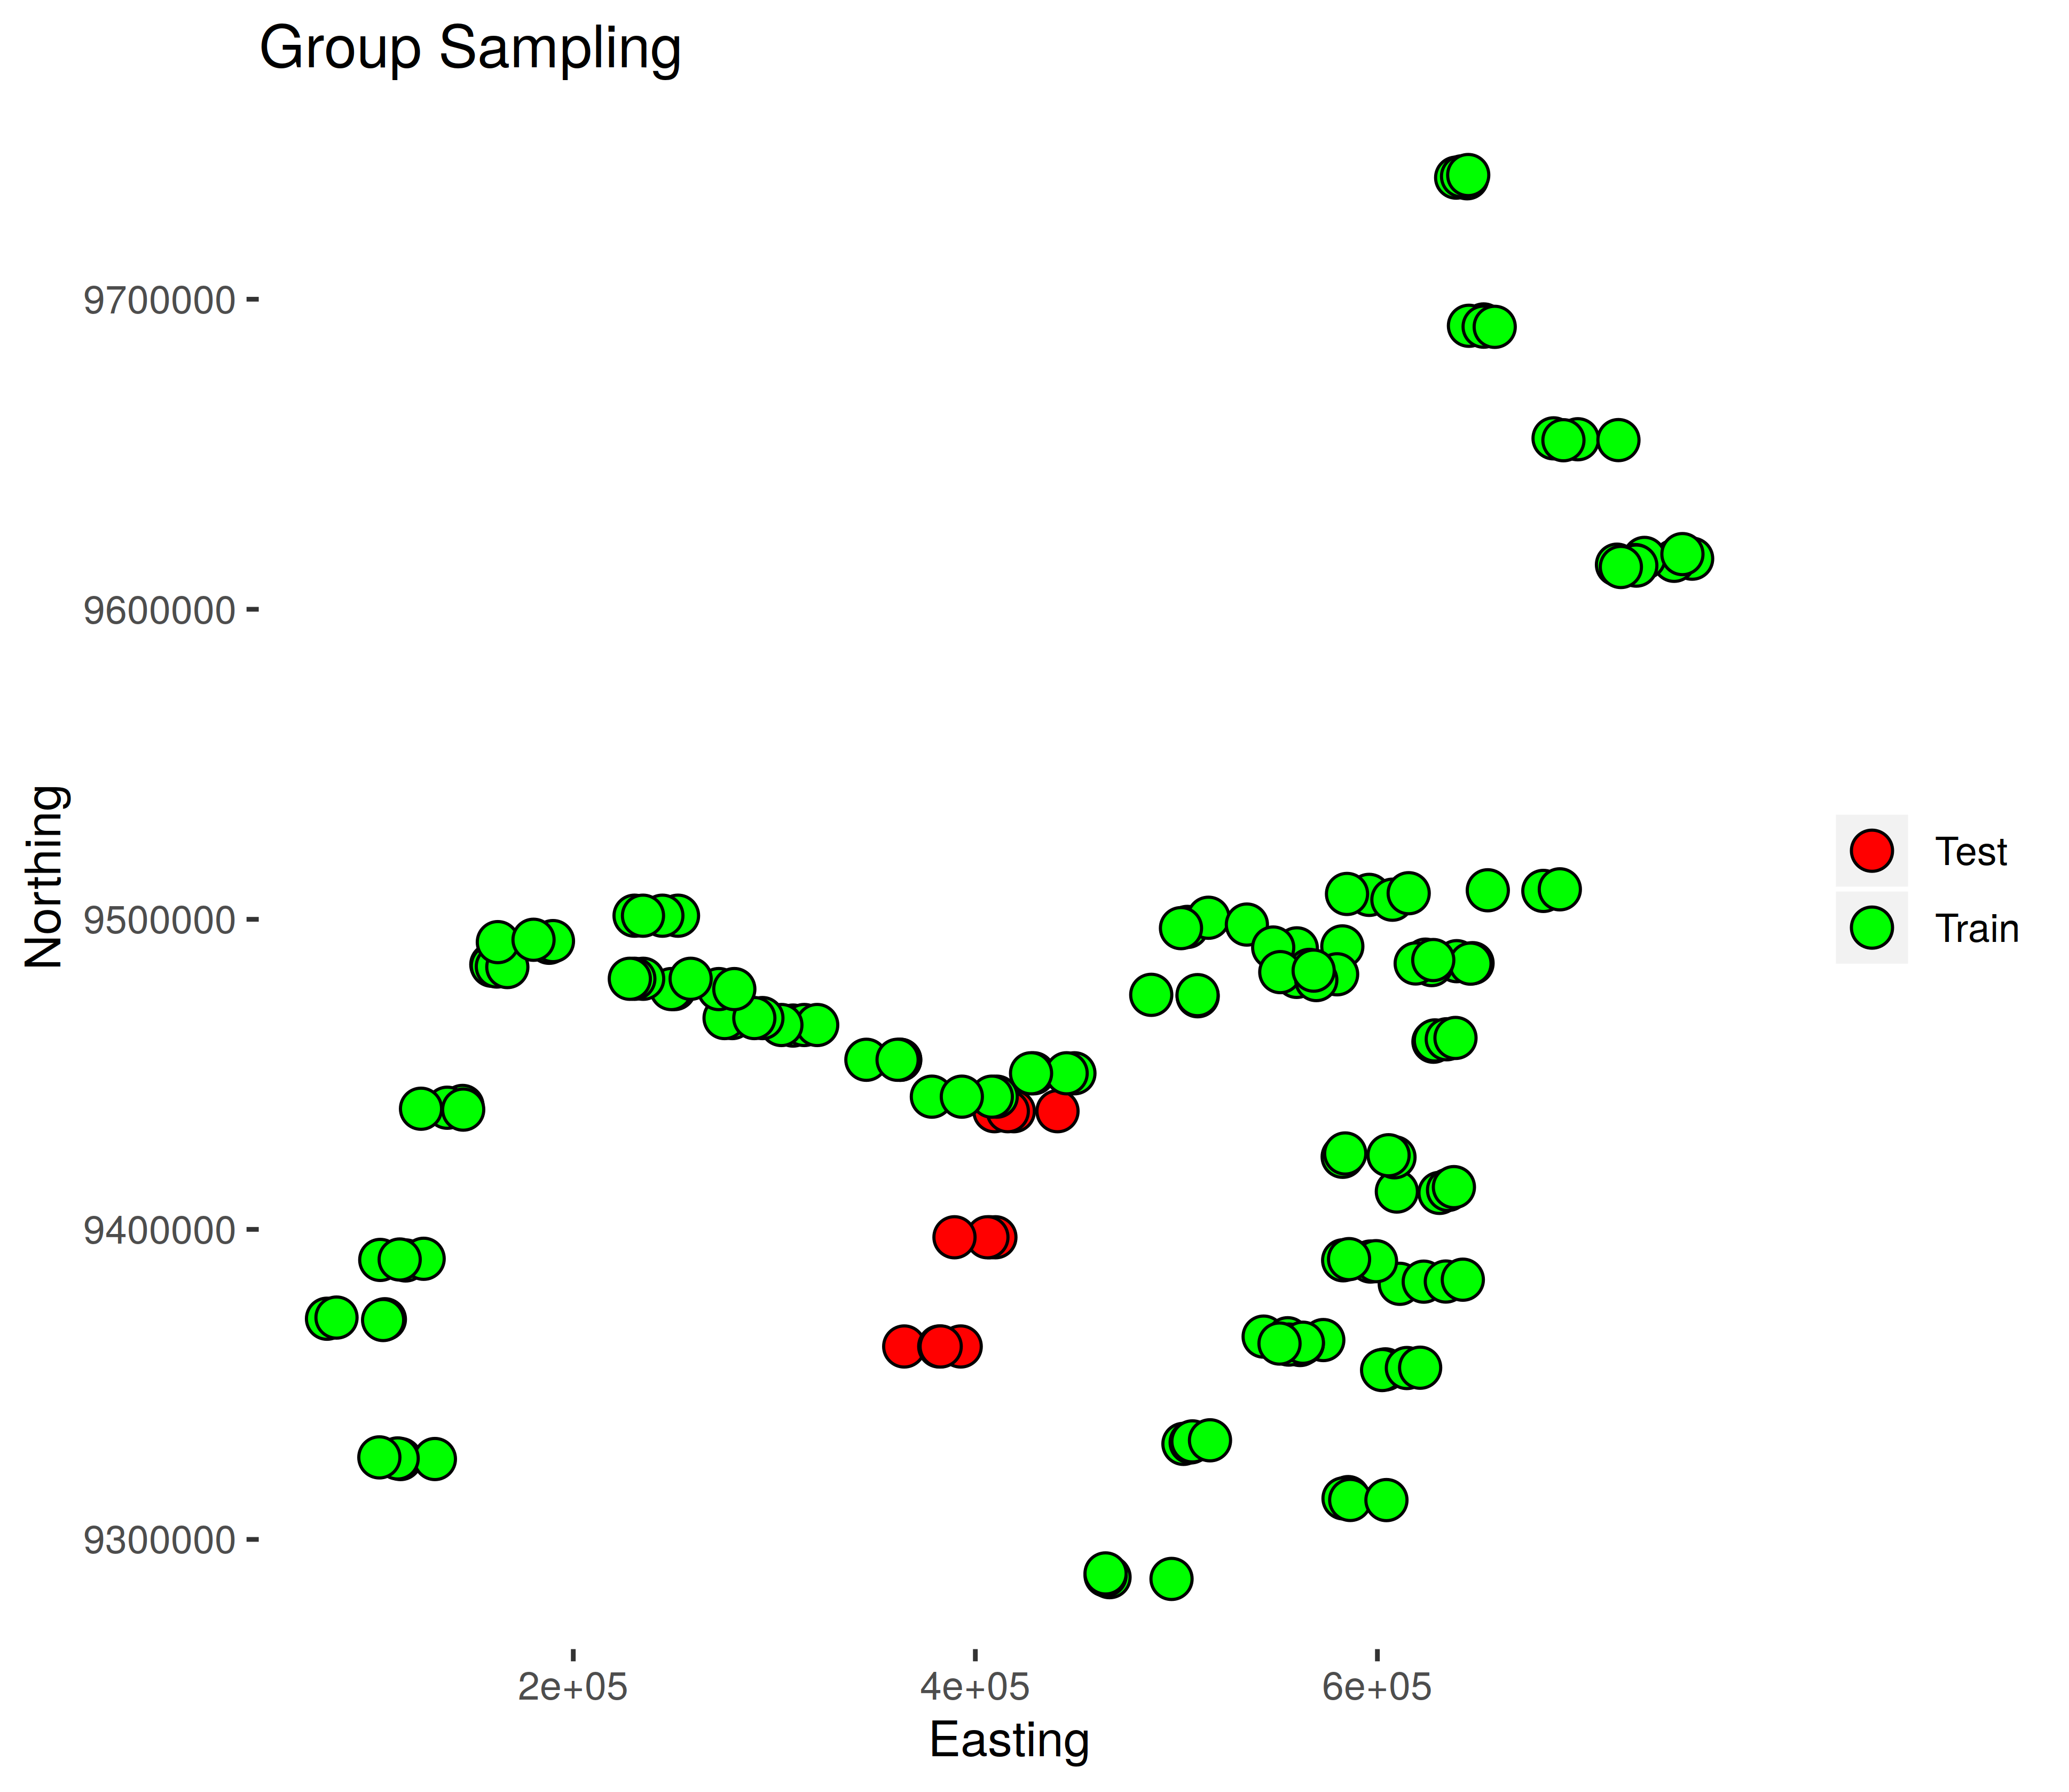
\includegraphics[width = \textwidth]{groupsamp2.png}
%\end{subfigure}
%\caption{Test set samples are geographically distinct from Train set samples. This represents a maximally dissimilar split which is created by choosing a different part of the river as the Testing set.}
%\label{fig:groupsamp}
%\end{figure}
%
%
%
%
%%Validation sets
%In addition to splitting the data into training and test sets, the train set was further split into validation sets so as to tune the hyperparameters of the models. The splitting into validation sets followed the same principle/method as the train-test split. So if, for example, the train and test sets were split using the maximally similar approach, the validation sets produced from the train set were chosen so as to be maximally similar to the remaining set.
%
%
%The steps of testing a classifier using a specific split method are as follows:
%\begin{enumerate}
%\item The data set is split into train and test sets based on the splitting method of choice. 
%\item The train set is split into $K$-folds using the same method for the train-test split.
%\item A set of hyperparameters and potential values are chosen for the cross-validation procedure. For example, in Logistic Regression a set of numbers ranging from 0.001 to 20 is chosen for the sparsity parameter and the set $\{True,False\}$ is chosen for the intercept parameter    
%\item The classifier is trained on the $K-1$ folds and tested on the remaining validation set for all possible combinations of hyperparameters (e.g. the Logistic Regressor is trained with hyperparameters $\{0.001,True\},\{0.001,False\},\{1.001,True\},\{1.001,False\}$ etc...).
%\item Step 4 is repeated for all the $K$-folds (by training on the $K-1$ and testing on the one left out). The average score across the validation sets is found for each hyperparameter combination and the classifier is retrained on the train set using the best hyperparameters set.
%\item The retrained model is tested on the test set and the prediction score is calculated.
%\item Steps  1 through 6 are repeated a number of times for different train-test splits using the same split principles. The scores for each repetition are stored.  
%\end{enumerate}
%
%This procedure can be repeated for different features (data sets), so as to evaluate how feature selection and transformations can alter the results. The best classifier for the particular features and splitting method is the one which has the highest mean score across all train-test splits. The various data sets used to test the classifiers on are summarised in table \ref{table:features}.
%\begin{table}
%	\caption{Features used in Classification}
%	\centering
%	\label{table:features}
%	\begin{tabularx}{\textwidth}{l X  }
%		\hline 
%		Features used &Description of dataset\\ 
%		
%		\hline
%		OTU &The OTU table as it is without any modifications done to it \\
%		OTU LOW & The OTU table without highly correlated features\\
%		OTU CSS & The normalised OTU table using CSS\\
%		OTU Min CSS & The normalised OTU table using CSS without samples with total counts of less than 10000 reads  \\
%		OTU CSS LOG & A $\log_2$ transformed OTU CSS \\
%		PCoA Bray-Curtis &The transformation of the OTU table with PCoA using the Bray-Curtis measure  \\
%		PCoA Bray-Curtis CSS &The transformation of the normalised OTU table with PCoA using the Bray-Curtis measure\\
%		
%		\hline 
%	\end{tabularx}
%\end{table}
%
%{ \large\bf Maximising Similarity} \\
%\textit{Aim}: Evaluate how well the classifiers perform when they are tested on a set which is similar geographically to the train set.\\
%\textit{Method}: Testing and validation sets are made up of samples coming from every part of the river. Care is taken to ensure that no geographical area is over represented. This is done using Stratified sampling (using the method StratifieKfold) where the strata (or groups) are the areas of the rivers the samples belong to. Stratified sampling ensures that the distribution of test or validation samples in each area is approximately the same as for train samples.
%
%
%
%
%{ \large \bf Maximising Dissimilarity}\\
%\textit{Aim}: Evaluate how well the classifiers perform when they are tested on a set which is dissimilar (or far away) geographically to the train set.\\
%\textit{Method}: Testing and Validation sets are made up of all the samples which belong to a particular area of the river. For example, the test set might be constituted by all the samples in the Upper Marañón area, and the validation sets by all the remaining areas (Huallaga, Min Maranon, Lower Maranon, Ucayali, Tapiche, Napo). The method used to produce these splits is called GroupKfold.
%
%{\large \bf Random Splits}\\
%\textit{Aim}: Evaluate the performance of the classifiers on train and test sets obtained by random splitting
%\textit{Method}: Test and Validation sets are obtained by randomly splitting the data. Care is taken to ensure that the balance of white and black water samples is the same across splits. This is done using Stratified sampling with the colour of the river as the strata.
%
%
%{ \bf Ideal Splits}
%An ideal sampling method would take into account the spatial correlation structures between the samples, besides just their location. Since the river flows eastwards from Maranon Upper down to all other streams, samples collected upstream would inevitably affect those from downstream, but the opposite might not be true. Thus, euclidean proximity of the river samples is not always a good enough indicator for detecting similarity between samples. For example, sample A collected near the opening of the Tapiche stream and sample B collected a bit further South of the opening, in the Ucayali stream, will have a smaller distance between them than with other samples collected further south in the Tapiche and Ucayaly streams. However, since the streams diverge, A and B might be more similar to samples found downstream their part of the river (Tapiche and Ucayaly respectively) than between them. 
%
%To achieve this, a directed graph of the river can be constructed, with vertices representing the samples, and edges the river path between them. Then a sampling scheme can take into account the stream direction and split the dataset in more sophisticated ways. One such way can test a classifier's ability to predict river colour if the test set is downstream from the train set, and the opposite, if the test set is upstream from the train. 
%
%
%%\begin{table}
%%\caption{Even better looking table using booktabs}
%%\centering
%%\label{table:good_table}
%%\begin{tabular}{l c c c c}
%%\toprule
%%\multirow{2}{*}{Dental measurement} & \multicolumn{2}{c}{Species I} & \multicolumn{2}{c}{Species II} \\ 
%%\cmidrule{2-5}
%%  & mean & SD  & mean & SD  \\ 
%%\midrule
%%I1MD & 6.23 & 0.91 & 5.2  & 0.7  \\
%%
%%I1LL & 7.48 & 0.56 & 8.7  & 0.71 \\
%%
%%I2MD & 3.99 & 0.63 & 4.22 & 0.54 \\
%%
%%I2LL & 6.81 & 0.02 & 6.66 & 0.01 \\
%%
%%CMD & 13.47 & 0.09 & 10.55 & 0.05 \\
%%
%%CBL & 11.88 & 0.05 & 13.11 & 0.04\\ 
%%\bottomrule
%%\end{tabular}
%%\end{table}


   %%%% HAMILTONIAN MCMC
\section{Hamiltonian Monte Carlo}
\label{section:hmc}
\subsection{Motivation}

Hamiltonian Monte carlo is a method for sampling from the distribution of interest, using properties of Hamiltonian dynamics. Because of the way new states are proposed in HMC, it can explore the state space faster (with less samples).

Usually the quantities we wish to evaluate in Bayesian Inference are the expectations of a function $f$ over the density of interest $p(q)$ in the parameter space $\mathcal{Q}$
\begin{equation}
	E_p(f) = \int_{\mathcal{Q}}p(q)f(q)dq.
\end{equation}

As was discussed previously, these integrals can be analytically intractable for any non-trivial target distribution, and that is why numerical methods are employed to approximate them. If the variation of the function of interest does not strongly affect the inegral, we might assume that most of it comes from the neighbourhood around the mode of the target density (where it is maximised).

This assumption however is misplaced, as the integral is calculated by accumulating the integrand over a volume of parameter space. The volume plays an increasingly important role the more dimensions of the parameter space we consider. This can be better understood by partitioning a parameters space into rectangles centred around the mode of the distribution. 

In one dimension, there are two partitions of our space, a line to the left and to the right of the mode. Thus it makes up for $1/3$ of the volume. In two dimensions we can fit eight squares/partitions around the mode, where it accounts for $1/9$th of the volume. In 3 dimensions, there are 26 partitions adjacent to the mode. If instead we consider the volume outside this neighbourhood of cubes, we find even more volume. 

We can conclude that most of the volume exists in the tails of the distribution of interest, far away form the mode, and it grows exponentially as the dimensions increase. Densities on the other hand have exactly the opposite property, since they have to integrate to unity (or a constant). 


Therefore, the regions of parameter space which contribute most to the expectation are not found either close to the mode, or very far away from it. These regions are usually called the typical set, which is found around the mode, and which is what we want to explore with an MCMC sampler. 


The method we need to explore the typical set should do it fast enough and not get stuck at pathological points of the distribution. The metropolis-hastings algorithm, given enough time, will explore most of the space of interest. However, because of the necessary exploration needed of the parameter set in states of low probability density, and the way the algorithm proposes and accepts new samples, the markov chain will rarely move. Because of limited computational power, a new method is needed that explores the typical set much faster.

This is where Hamiltonian dynamics becomes useful. The problem of exploring the typical set can be recast into a physics problem; the orbit of a satellite around a planet. The gravitational potential energy exerted by the planet can be viewed as the target density. Its gradient points towards the planet and thus going along it will cause the satellite to crash. To keep it in orbit we have to pump it with enough momentum to keep it going around the planet, but also not too much so that it flies away to the depths of space. Because of the conservative dynamics of this system, giving the satellite just enough energy at the start of the orbit will keep it at approximately the same zone.

The key to exploring the typical set, is thus by introducing auxiliary momentum parameters to our probabilistic system. They have to be added, however in such a way that the conservative dynamics of the system are ensured.

\subsection{Formulation}

The Hamiltonian of a system is completely defined by its position $q_i$ and momentum $p_i$, and it describes how these variables change with time 
\begin{align}
	\frac{dq_i}{dt} &= \frac{\partial H}{\partial p_i}\nonumber\\
		\frac{dp_i}{dt} &= -\frac{\partial H}{\partial q_i} \label{eq:motion}
\end{align}
It can be expressed as the sum of the potential $U(q)$ and kinetic $K(p)$ energy
\begin{equation}
	H(q,p) = U(q) + K(p).
\end{equation}
and thus the equations of motion can be rewritten to 
\begin{align}
\frac{dq_i}{dt} &= \frac{\partial K}{\partial p_i}\nonumber\\
\frac{dp_i}{dt} &= -\frac{\partial U}{\partial q_i} \label{eq:motion_kinetic_potential}
\end{align}

In the HMC, position variables $q$ denote the parameters of interest and the potential energy is the minus of the log of the target density. The kinetic energy is usually defined as 
\begin{equation}
	K(p)= \frac{p^T M^{-1}p}{2},
\end{equation}
where $M$ is a symmetric positive-definite matrix which is usually a diagonal multiplied by a constant. In probabilistic terms, the momentum variables have a multivariate normal distribution with $M$ as the covariance matrix.



The dynamics of the system satisfy some important properties without which the construction of valid MCMC updates would not be possible. First of all, the Hamiltonian of the system is time invariant 
\begin{equation}
	\frac{d H}{d t}=\sum_{i=1}^{d}\left[\frac{d q_{i}}{d t} \frac{\partial H}{\partial q_{i}}+\frac{d p_{i}}{d t} \frac{\partial H}{\partial p_{i}}\right]=\sum_{i=1}^{d}\left[\frac{\partial H}{\partial p_{i}} \frac{\partial H}{\partial q_{i}}-\frac{\partial H}{\partial q_{i}} \frac{\partial H}{\partial p_{i}}\right]=0.
\end{equation}
Another fundamental property is that the dynamics are reversible; there is a one-to-one map from the state $(q(t),p(t))$ at time $t$ to the state $(q(t+s),p(t+s))$ at time $t+s$, and thus the reverse map exists as well.
Finally, the phase space's $(q,p)$ volume is conserved, therefore, any mapping from one region in the phase space to another must conserve the initial volume. 


The introduction of the auxiliary momentum variables transforms the target distribution into a joint one in phase space 
\begin{equation}
	P(q,p) = P(p|q)P(q) = P(p)P(q).
\end{equation}
The joint density is equal to the probability of momentum given the position times the target distribution. This can be further simplified to the product of the two marginals, since we do not assume any dependence of the momentum to the position. The joint probability is related to the Hamiltonian via a canonical distribution
\begin{equation}
	P(q,p) = \frac{1}{Z}exp\left(-H(q,p)\right),
\end{equation}
where $Z$ is th normalising constant. 
Therefore we can rewrite the density as 
\begin{equation}
	P(q, p)=\frac{1}{Z} \exp \left({-U(q)}\right) \exp \left({-K(p)}\right).
\end{equation}
Under this formulation, we can see how the potential energy $U(q)$ can be viewed as the negative log of the target density 
\begin{equation}
	U(q) = -\log(p(q)).
\end{equation}

The kinetic energy on the other hand can take the form 
\begin{equation}
K(p)= \frac{p^T M^{-1}p}{2},
\end{equation}
where $M$ is a symmetric positive-definite matrix which is usually a diagonal multiplied by a constant. This is the usual definition of kinetic energy in physics, but under our probabilistic perspective (and the canonical distribution) it can be viewed as a multivariate Gaussian distribution over the momentum particles, centred at zero and with covariance matrix $M$. The partial derivative of the kinetic energy with respect to momentum $p_i$ is given by
\begin{equation}
	\frac{\partial K(p)}{\partial p_i} = [M^{-1}p]_i = \frac{p_i}{m_i}.
\end{equation}
The last equality is given when the covariance (mass) matrix is diagonal with $m_i$ as its $i$th diagonal element. 

Any trajectory in the phase space satisfying Hamilton's equations and the dynamics of the system leaves the joint probability density constant. Therefore, to draw samples of position from a previously unexplored region of phase space, we could generate a random momentum vector and use the previous value of the position. Then we could evolve the state $(q,p)$ using Hamilton's equations \eqref{eq:motion} until we reach the desired space, and accept the new samples. The process can be repeated by generating a new random momentum vector.


The problem with this method is that Hamilton's equations must be approximated by descritising them in time. Then the evolution of states is from time $t$ $(q(t),p(t))$ to time $t+\epsilon$ $(q(t+\epsilon),p(t+\epsilon))$, and whatever numerical method we use to do this, will not be perfect and have some numerical errors. The method most commonly used is the leapfrog which evolves in time the momentum variable first by half a step, then the position by a whole step using the evolved momentum, and finally completes the evolution of the momentum by one more half step
\begin{align}
 p_{i}(t+\varepsilon / 2) &=p_{i}(t)-(\varepsilon / 2) \frac{\partial U}{\partial q_{i}}(q(t)) \\ q_{i}(t+\varepsilon) &=q_{i}(t)+\varepsilon \frac{p_{i}(t+\varepsilon / 2)}{m_{i}} \\ p_{i}(t+\varepsilon) &=p_{i}(t+\varepsilon / 2)-(\varepsilon / 2) \frac{\partial U}{\partial a_{i}}(q(t+\varepsilon)) .
\end{align}

Because of numerical approximation errors, the new state $q^*$ found by the evolution of the Hamiltonian using the leapfrog method is accepted with a probability of 
\begin{equation}
	\text{acceptance probability of new state} = \min(1,\exp \left(H(q,p) - H(q^*,p^*)\right) ).
	\label{eq:acceptanceprobability}
\end{equation}
If the proposed state is not accepted then the next state is set to the current one. 

The algorithm starts with a specified initial set of parameters $q$, that can be predetermined or randomly generated. For every iteration of the algorithm new momentum $p$ parameters are generated and, together with the current $q$, are updated according to Hamiltonian dynamics using the leapfrog method performed $L$ number of times with discretisation time $\epsilon$. A metropolis acceptance step is then applied with probability \eqref{eq:acceptanceprobability}; if the new state $q^*$ of the parameter is accepted then it is appended to the markov chain. If the new state is not accepted then the previous values are used again. 

A crucial part of the method is the random generation of new momentum vector at each iteration. It is what moves the chain to $(q,p)$ points with different joint density, thus allowing for state phase exploration. The generation of new momentum for each step can change the density by a large amount, thus producing $q$ values with a much different density.

A more extensive treatment and some theoretical results can be found in Chapter 5 of the MCMC Handbook \cite{brooks_mcmc_2011}. For a conceptual introduction to the matter see \cite{betancourt_conceptual_2017}.


%\begin{algorithm}[H]
%	\SetAlgoLined
%	\KwReturn{A vector of the parameters of interest }
%	
%	\While{the number of samples obtained is less than $B$}{
%		instructions\;
%		\eIf{condition}{
%			instructions1\;
%			instructions2\;
%		}{
%			instructions3\;
%		}
%	}
%	\caption{Hamiltonian Monte Carlo samples}
%\end{algorithm}
%
%
%\begin{algorithm}[H]
%	\SetAlgoLined
%	\DontPrintSemicolon
%	\KwIn{}    
%	\KwOut{$ S^{*} $ \Comment*[r]{Negation Excluded List}}
%	
%	\SetKwFunction{FMain}{HMC Step}
%	\SetKwProg{Fn}{Function}{:}{}
%	\Fn{\FMain{U,grad_U,epsilon,L,current_q}}{
%		$q = current_q$
%		$p = \mathcal{N}(length(q),mean =0,sd=1)$    
%		$q,p = \text{Leapfrog_update}$
%		
%		current_U = U(current_q)
%		
%		\textbf{return} $ S^{*}; $ 
%	}
%	\textbf{End Function}
%	\caption{Algorithm for Excluding the Negation}
%	\label{NagetionAlgo}
%\end{algorithm}